\documentclass[twoside]{book}

% Packages required by doxygen
\usepackage{fixltx2e}
\usepackage{calc}
\usepackage{doxygen}
\usepackage[export]{adjustbox} % also loads graphicx
\usepackage{graphicx}
\usepackage[utf8]{inputenc}
\usepackage{makeidx}
\usepackage{multicol}
\usepackage{multirow}
\PassOptionsToPackage{warn}{textcomp}
\usepackage{textcomp}
\usepackage[nointegrals]{wasysym}
\usepackage[table]{xcolor}

% Font selection
\usepackage[T1]{fontenc}
\usepackage[scaled=.90]{helvet}
\usepackage{courier}
\usepackage{amssymb}
\usepackage{sectsty}
\renewcommand{\familydefault}{\sfdefault}
\allsectionsfont{%
  \fontseries{bc}\selectfont%
  \color{darkgray}%
}
\renewcommand{\DoxyLabelFont}{%
  \fontseries{bc}\selectfont%
  \color{darkgray}%
}
\newcommand{\+}{\discretionary{\mbox{\scriptsize$\hookleftarrow$}}{}{}}

% Page & text layout
\usepackage{geometry}
\geometry{%
  a4paper,%
  top=2.5cm,%
  bottom=2.5cm,%
  left=2.5cm,%
  right=2.5cm%
}
\tolerance=750
\hfuzz=15pt
\hbadness=750
\setlength{\emergencystretch}{15pt}
\setlength{\parindent}{0cm}
\setlength{\parskip}{3ex plus 2ex minus 2ex}
\makeatletter
\renewcommand{\paragraph}{%
  \@startsection{paragraph}{4}{0ex}{-1.0ex}{1.0ex}{%
    \normalfont\normalsize\bfseries\SS@parafont%
  }%
}
\renewcommand{\subparagraph}{%
  \@startsection{subparagraph}{5}{0ex}{-1.0ex}{1.0ex}{%
    \normalfont\normalsize\bfseries\SS@subparafont%
  }%
}
\makeatother

% Headers & footers
\usepackage{fancyhdr}
\pagestyle{fancyplain}
\fancyhead[LE]{\fancyplain{}{\bfseries\thepage}}
\fancyhead[CE]{\fancyplain{}{}}
\fancyhead[RE]{\fancyplain{}{\bfseries\leftmark}}
\fancyhead[LO]{\fancyplain{}{\bfseries\rightmark}}
\fancyhead[CO]{\fancyplain{}{}}
\fancyhead[RO]{\fancyplain{}{\bfseries\thepage}}
\fancyfoot[LE]{\fancyplain{}{}}
\fancyfoot[CE]{\fancyplain{}{}}
\fancyfoot[RE]{\fancyplain{}{\bfseries\scriptsize Generated by Doxygen }}
\fancyfoot[LO]{\fancyplain{}{\bfseries\scriptsize Generated by Doxygen }}
\fancyfoot[CO]{\fancyplain{}{}}
\fancyfoot[RO]{\fancyplain{}{}}
\renewcommand{\footrulewidth}{0.4pt}
\renewcommand{\chaptermark}[1]{%
  \markboth{#1}{}%
}
\renewcommand{\sectionmark}[1]{%
  \markright{\thesection\ #1}%
}

% Indices & bibliography
\usepackage{natbib}
\usepackage[titles]{tocloft}
\setcounter{tocdepth}{3}
\setcounter{secnumdepth}{5}
\makeindex

% Hyperlinks (required, but should be loaded last)
\usepackage{ifpdf}
\ifpdf
  \usepackage[pdftex,pagebackref=true]{hyperref}
\else
  \usepackage[ps2pdf,pagebackref=true]{hyperref}
\fi
\hypersetup{%
  colorlinks=true,%
  linkcolor=blue,%
  citecolor=blue,%
  unicode%
}

% Custom commands
\newcommand{\clearemptydoublepage}{%
  \newpage{\pagestyle{empty}\cleardoublepage}%
}

\usepackage{caption}
\captionsetup{labelsep=space,justification=centering,font={bf},singlelinecheck=off,skip=4pt,position=top}

%===== C O N T E N T S =====

\begin{document}

% Titlepage & ToC
\hypersetup{pageanchor=false,
             bookmarksnumbered=true,
             pdfencoding=unicode
            }
\pagenumbering{alph}
\begin{titlepage}
\vspace*{7cm}
\begin{center}%
{\Large F\+O\+S\+S\+A\+S\+A\+T-\/1 Ground Station }\\
\vspace*{1cm}
{\large Generated by Doxygen 1.8.14}\\
\end{center}
\end{titlepage}
\clearemptydoublepage
\pagenumbering{roman}
\tableofcontents
\clearemptydoublepage
\pagenumbering{arabic}
\hypersetup{pageanchor=true}

%--- Begin generated contents ---
\chapter{Main Page}
\label{index}\hypertarget{index}{}\hypertarget{index_sec_1}{}\section{About}\label{index_sec_1}


 The ground station is the system that is distributed to lots of users. It receives and transmists messages to the satellite and also performs auto-\/tuning functions and relays messages to a central storage server.

The target for this is a stand alone system with simple IO and connection to the internet.\hypertarget{index_sec_2}{}\section{The Transmission Protocol}\label{index_sec_2}


 \hypertarget{index_Restrictions}{}\subsection{Restrictions}\label{index_Restrictions}

\begin{DoxyItemize}
\item Max send length of a string 256 characters.
\item 512 bytes in total
\end{DoxyItemize}\hypertarget{index_Format}{}\subsection{Format}\label{index_Format}
1 byte = function id (0-\/256) 511 bytes = message of any format\hypertarget{index_Function}{}\subsection{I\+D Descriptors}\label{index_Function}
\hypertarget{index_multi_row}{}
\tabulinesep=1mm
\begin{longtabu} spread 0pt [c]{*{4}{|X[-1]}|}
\caption{See the {\ttfamily communications.\+cpp} doxygen documentation page for info on where the transmissions are set from within the software.}\label{index_multi_row}\\
\hline
\rowcolor{\tableheadbgcolor}\textbf{ Function ID (character type) }&\textbf{ Direction Bound }&\textbf{ Description }&\textbf{ Received Type  }\\\cline{1-4}
\endfirsthead
\hline
\endfoot
\hline
\rowcolor{\tableheadbgcolor}\textbf{ Function ID (character type) }&\textbf{ Direction Bound }&\textbf{ Description }&\textbf{ Received Type  }\\\cline{1-4}
\endhead
1 &To Ground &Arduino has started. &No data sent  \\\cline{1-4}
2 &To Ground &Arduino has stopped. &No data sent  \\\cline{1-4}
3 &To Ground &Satellite transceiver online &No data sent  \\\cline{1-4}
4 &To Ground &Solar panel and antenna deployment successful. &No data sent  \\\cline{1-4}
5 &To Satellite &Invoke P\+I\+NG on satellite. &No data sent  \\\cline{1-4}
6 &To Ground &Reply to P\+I\+NG (\char`\"{}5\char`\"{}) with P\+O\+NG transmission. &No data sent  \\\cline{1-4}
7 &To Satellite &Stop transmitting. &No data sent  \\\cline{1-4}
8 &To Satellite &Start transmitting. &No data sent  \\\cline{1-4}
9 &To Ground &Transmit system power, reset count and deployment status infomation to the ground. &S\+T\+R\+I\+NG \+: \char`\"{}\+S1\+:int;\+S2\+:int;\+S3\+:int;\+S4\+:int;\+S5\+:int;\+R\+C\+:int;\+D\+E\+P\+S\+:int;\char`\"{}  \\\cline{1-4}
10 &To Ground &Transmit system tuning and configuration message. &S\+T\+R\+I\+NG \+: \char`\"{}\+F\+O\+S\+S\+A\+S\+A\+T1\char`\"{}  \\\cline{1-4}
\end{longtabu}


 
\chapter{Test List}
\label{test}
\Hypertarget{test}

\begin{DoxyRefList}
\item[\label{test__test000001}%
\Hypertarget{test__test000001}%
Member \mbox{\hyperlink{communication_8h_a68fd88d1ccfc91925d30c0fdf1b417ab}{Communication\+\_\+\+S\+X1278\+Transmit}} (String in\+Func\+Id, String in\+Message)]in\+Func\+Id range String(-\/inf) to String(inf). 

in\+Func\+Id String length above 256 

In\+Func\+Id empty string. 

in\+Message String empty. 

in\+Message length above 256.  
\item[\label{test__test000003}%
\Hypertarget{test__test000003}%
Member \mbox{\hyperlink{ground__station_8cpp_afe461d27b9c48d5921c00d521181f12f}{loop}} ()]See how it behaves without a S\+X1278 interface. 

Test each function ID and ensure it prints to debug the correct functions. 

Ensure that the frequency error we receive on a packet is suitable for tuning with. 

Does changing the frequency of the L\+O\+RA class at runtime work? 

D\+Oes changing the bandwidth of the L\+O\+RA class at runtime work?  
\item[\label{test__test000002}%
\Hypertarget{test__test000002}%
Member \mbox{\hyperlink{ground__station_8cpp_a4fc01d736fe50cf5b977f755b675f11d}{setup}} ()]Test ground station with no S\+X1278 chip connected to see how it fails. 
\end{DoxyRefList}
\chapter{Todo List}
\label{todo}
\Hypertarget{todo}

\begin{DoxyRefList}
\item[\label{todo__todo000004}%
\Hypertarget{todo__todo000004}%
Member \mbox{\hyperlink{communication_8h_a649fe6cc16cc68a0eda736de6d670ea4}{Communication\+\_\+\+Received\+Deployment\+Success}} ()]Implement satellite deployment success signal.  
\item[\label{todo__todo000002}%
\Hypertarget{todo__todo000002}%
Member \mbox{\hyperlink{communication_8h_ab24ce0353afa549bb631933e8cfe9343}{Communication\+\_\+\+Received\+Stopped\+Signal}} ()]Implement satellite stop signal transmission.  
\item[\label{todo__todo000003}%
\Hypertarget{todo__todo000003}%
Member \mbox{\hyperlink{communication_8h_a9120f84592164d2c696fc5d8b9948ac1}{Communication\+\_\+\+Received\+Transmitted\+Online}} ()]Add output interface. 

Implement satellite stop signal transmission. 
\item[\label{todo__todo000001}%
\Hypertarget{todo__todo000001}%
Member \mbox{\hyperlink{communication_8h_a68fd88d1ccfc91925d30c0fdf1b417ab}{Communication\+\_\+\+S\+X1278\+Transmit}} (String in\+Func\+Id, String in\+Message)]Debug Logging removal. 

Transmission signature containment.  
\item[\label{todo__todo000005}%
\Hypertarget{todo__todo000005}%
Member \mbox{\hyperlink{communication_8h_a639d7624642ba6e8f368f15b89d1b557}{Communication\+\_\+\+Transmit\+Ping}} ()]Implement user interface for ground station.  
\item[\label{todo__todo000007}%
\Hypertarget{todo__todo000007}%
Member \mbox{\hyperlink{communication_8h_aa11cefca5402f3a480be0b8448916dab}{Communication\+\_\+\+Transmit\+Start\+Transmitting}} ()]Reference the security code that requires this functionality.  
\item[\label{todo__todo000006}%
\Hypertarget{todo__todo000006}%
Member \mbox{\hyperlink{communication_8h_a7d368a63e53f4a1a63b166e6e97c7805}{Communication\+\_\+\+Transmit\+Stop\+Transmitting}} ()]Reference the security code that requires this functionality. 
\end{DoxyRefList}
\chapter{File Index}
\section{File List}
Here is a list of all files with brief descriptions\+:\begin{DoxyCompactList}
\item\contentsline{section}{\mbox{\hyperlink{communication_8cpp}{communication.\+cpp}} \\*This code manages the protocol transmission. It takes raw values from the system, packs them into the radio protocol and sends it through the S\+X1278 }{\pageref{communication_8cpp}}{}
\item\contentsline{section}{\mbox{\hyperlink{communication_8h}{communication.\+h}} }{\pageref{communication_8h}}{}
\item\contentsline{section}{\mbox{\hyperlink{configuration_8cpp}{configuration.\+cpp}} \\*This is the file in which all the static flags are stored. these are to be switched during prototype development }{\pageref{configuration_8cpp}}{}
\item\contentsline{section}{\mbox{\hyperlink{configuration_8h}{configuration.\+h}} }{\pageref{configuration_8h}}{}
\item\contentsline{section}{\mbox{\hyperlink{debugging__utilities_8cpp}{debugging\+\_\+utilities.\+cpp}} \\*Serial println abstraction with D\+E\+B\+UG configuration switch. This is so all printlns can be traced }{\pageref{debugging__utilities_8cpp}}{}
\item\contentsline{section}{\mbox{\hyperlink{debugging__utilities_8h}{debugging\+\_\+utilities.\+h}} }{\pageref{debugging__utilities_8h}}{}
\item\contentsline{section}{\mbox{\hyperlink{ground__station_8cpp}{ground\+\_\+station.\+cpp}} \\*This is the main code starting point. It manages the state of the ground station }{\pageref{ground__station_8cpp}}{}
\item\contentsline{section}{\mbox{\hyperlink{state__machine__declerations_8cpp}{state\+\_\+machine\+\_\+declerations.\+cpp}} \\*Where the state machine booleans are held for easy access }{\pageref{state__machine__declerations_8cpp}}{}
\item\contentsline{section}{\mbox{\hyperlink{state__machine__declerations_8h}{state\+\_\+machine\+\_\+declerations.\+h}} }{\pageref{state__machine__declerations_8h}}{}
\end{DoxyCompactList}

\chapter{File Documentation}
\hypertarget{communication_8cpp}{}\section{communication.\+cpp File Reference}
\label{communication_8cpp}\index{communication.\+cpp@{communication.\+cpp}}


This code manages the protocol transmission. It takes raw values from the system, packs them into the radio protocol and sends it through the S\+X1278.  


{\ttfamily \#include \char`\"{}configuration.\+h\char`\"{}}\newline
{\ttfamily \#include \char`\"{}state\+\_\+machine\+\_\+declerations.\+h\char`\"{}}\newline
{\ttfamily \#include \char`\"{}communication.\+h\char`\"{}}\newline
{\ttfamily \#include \char`\"{}debugging\+\_\+utilities.\+h\char`\"{}}\newline
Include dependency graph for communication.\+cpp\+:\nopagebreak
\begin{figure}[H]
\begin{center}
\leavevmode
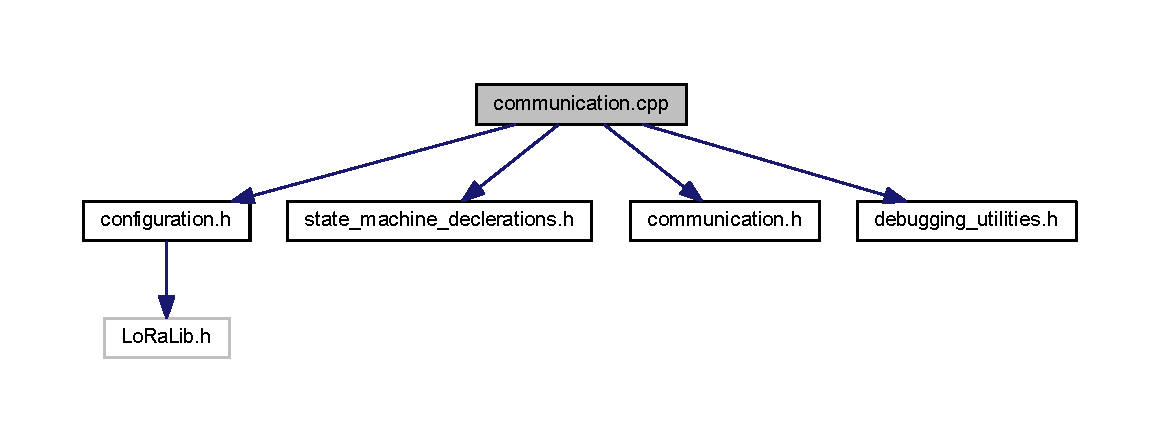
\includegraphics[width=350pt]{communication_8cpp__incl}
\end{center}
\end{figure}
\subsection*{Functions}
\begin{DoxyCompactItemize}
\item 
void \mbox{\hyperlink{communication_8cpp_a68fd88d1ccfc91925d30c0fdf1b417ab}{Communication\+\_\+\+S\+X1278\+Transmit}} (String in\+Func\+Id, String in\+Message)
\item 
void \mbox{\hyperlink{communication_8cpp_ab66ce78f3bfe62d6583da0a1a1473e6b}{Communication\+\_\+\+Received\+Started\+Signal}} ()
\item 
void \mbox{\hyperlink{communication_8cpp_ab24ce0353afa549bb631933e8cfe9343}{Communication\+\_\+\+Received\+Stopped\+Signal}} ()
\item 
void \mbox{\hyperlink{communication_8cpp_a9120f84592164d2c696fc5d8b9948ac1}{Communication\+\_\+\+Received\+Transmitted\+Online}} ()
\item 
void \mbox{\hyperlink{communication_8cpp_a649fe6cc16cc68a0eda736de6d670ea4}{Communication\+\_\+\+Received\+Deployment\+Success}} ()
\item 
void \mbox{\hyperlink{communication_8cpp_ad67fe0fd5088334be55f2045f5c2067f}{Communication\+\_\+\+Received\+Pong}} ()
\item 
void \mbox{\hyperlink{communication_8cpp_a639d7624642ba6e8f368f15b89d1b557}{Communication\+\_\+\+Transmit\+Ping}} ()
\item 
void \mbox{\hyperlink{communication_8cpp_a7d368a63e53f4a1a63b166e6e97c7805}{Communication\+\_\+\+Transmit\+Stop\+Transmitting}} ()
\item 
void \mbox{\hyperlink{communication_8cpp_aa11cefca5402f3a480be0b8448916dab}{Communication\+\_\+\+Transmit\+Start\+Transmitting}} ()
\item 
void \mbox{\hyperlink{communication_8cpp_a9dd32118d0d9d6eaa0cf4c5646622549}{Communication\+\_\+\+Received\+Power\+Info}} (String in\+Message)
\item 
void \mbox{\hyperlink{communication_8cpp_a18e4470849a0b104b638efb80f2f56d7}{Communication\+\_\+\+Received\+Transceiver\+Settings}} (String in\+Message, float in\+Frequency\+Error)
\end{DoxyCompactItemize}


\subsection{Detailed Description}
This code manages the protocol transmission. It takes raw values from the system, packs them into the radio protocol and sends it through the S\+X1278. 



\subsection{Function Documentation}
\mbox{\Hypertarget{communication_8cpp_a649fe6cc16cc68a0eda736de6d670ea4}\label{communication_8cpp_a649fe6cc16cc68a0eda736de6d670ea4}} 
\index{communication.\+cpp@{communication.\+cpp}!Communication\+\_\+\+Received\+Deployment\+Success@{Communication\+\_\+\+Received\+Deployment\+Success}}
\index{Communication\+\_\+\+Received\+Deployment\+Success@{Communication\+\_\+\+Received\+Deployment\+Success}!communication.\+cpp@{communication.\+cpp}}
\subsubsection{\texorpdfstring{Communication\+\_\+\+Received\+Deployment\+Success()}{Communication\_ReceivedDeploymentSuccess()}}
{\footnotesize\ttfamily void Communication\+\_\+\+Received\+Deployment\+Success (\begin{DoxyParamCaption}{ }\end{DoxyParamCaption})}

Called when received Function ID \char`\"{}4\char`\"{}.

This function indicates to the ground station that the deployment sequence was successfull.

Received\+: Satellite\textquotesingle{}s Setup() function.

\begin{DoxyRefDesc}{Todo}
\item[\mbox{\hyperlink{todo__todo000004}{Todo}}]Implement satellite deployment success signal. \end{DoxyRefDesc}
Here is the call graph for this function\+:\nopagebreak
\begin{figure}[H]
\begin{center}
\leavevmode
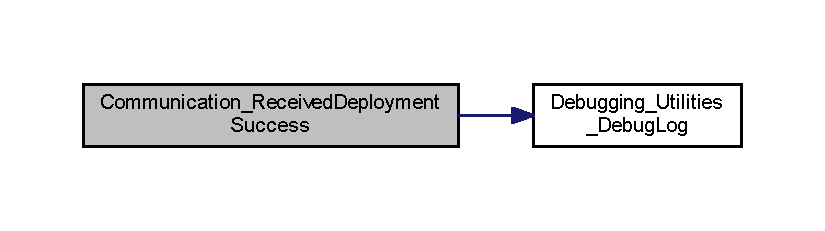
\includegraphics[width=350pt]{communication_8cpp_a649fe6cc16cc68a0eda736de6d670ea4_cgraph}
\end{center}
\end{figure}
Here is the caller graph for this function\+:\nopagebreak
\begin{figure}[H]
\begin{center}
\leavevmode
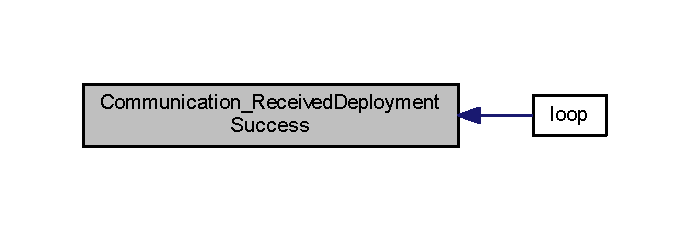
\includegraphics[width=331pt]{communication_8cpp_a649fe6cc16cc68a0eda736de6d670ea4_icgraph}
\end{center}
\end{figure}
\mbox{\Hypertarget{communication_8cpp_ad67fe0fd5088334be55f2045f5c2067f}\label{communication_8cpp_ad67fe0fd5088334be55f2045f5c2067f}} 
\index{communication.\+cpp@{communication.\+cpp}!Communication\+\_\+\+Received\+Pong@{Communication\+\_\+\+Received\+Pong}}
\index{Communication\+\_\+\+Received\+Pong@{Communication\+\_\+\+Received\+Pong}!communication.\+cpp@{communication.\+cpp}}
\subsubsection{\texorpdfstring{Communication\+\_\+\+Received\+Pong()}{Communication\_ReceivedPong()}}
{\footnotesize\ttfamily void Communication\+\_\+\+Received\+Pong (\begin{DoxyParamCaption}{ }\end{DoxyParamCaption})}

Called when received Function ID \char`\"{}6\char`\"{}.

This function indicates to the ground station that the satellite received the Ping transmission.

Received\+: Satellite receives Ping function \char`\"{}5\char`\"{} transmission. Here is the call graph for this function\+:\nopagebreak
\begin{figure}[H]
\begin{center}
\leavevmode
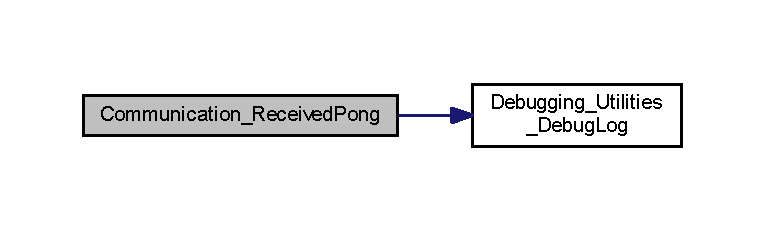
\includegraphics[width=350pt]{communication_8cpp_ad67fe0fd5088334be55f2045f5c2067f_cgraph}
\end{center}
\end{figure}
Here is the caller graph for this function\+:\nopagebreak
\begin{figure}[H]
\begin{center}
\leavevmode
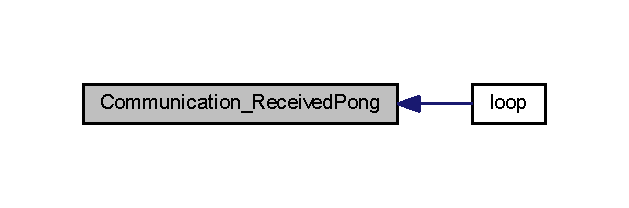
\includegraphics[width=302pt]{communication_8cpp_ad67fe0fd5088334be55f2045f5c2067f_icgraph}
\end{center}
\end{figure}
\mbox{\Hypertarget{communication_8cpp_a9dd32118d0d9d6eaa0cf4c5646622549}\label{communication_8cpp_a9dd32118d0d9d6eaa0cf4c5646622549}} 
\index{communication.\+cpp@{communication.\+cpp}!Communication\+\_\+\+Received\+Power\+Info@{Communication\+\_\+\+Received\+Power\+Info}}
\index{Communication\+\_\+\+Received\+Power\+Info@{Communication\+\_\+\+Received\+Power\+Info}!communication.\+cpp@{communication.\+cpp}}
\subsubsection{\texorpdfstring{Communication\+\_\+\+Received\+Power\+Info()}{Communication\_ReceivedPowerInfo()}}
{\footnotesize\ttfamily void Communication\+\_\+\+Received\+Power\+Info (\begin{DoxyParamCaption}\item[{String}]{in\+Message }\end{DoxyParamCaption})}

Function ID \char`\"{}9\char`\"{}.

This function is called when the ground station receives a power infomation transmission. The power info is broadcasted every 400s.

Received\+: every 400ms from the satellite\textquotesingle{}s Loop(). Here is the call graph for this function\+:\nopagebreak
\begin{figure}[H]
\begin{center}
\leavevmode
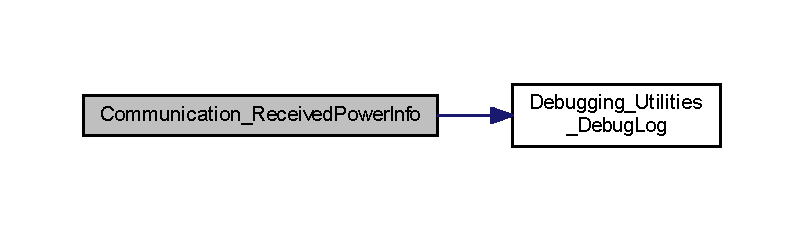
\includegraphics[width=350pt]{communication_8cpp_a9dd32118d0d9d6eaa0cf4c5646622549_cgraph}
\end{center}
\end{figure}
Here is the caller graph for this function\+:\nopagebreak
\begin{figure}[H]
\begin{center}
\leavevmode
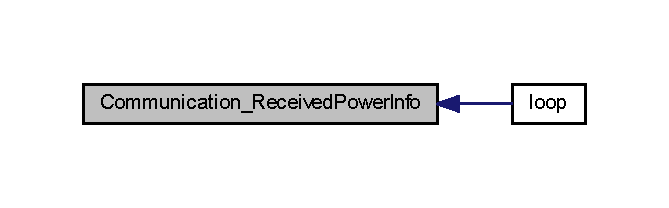
\includegraphics[width=321pt]{communication_8cpp_a9dd32118d0d9d6eaa0cf4c5646622549_icgraph}
\end{center}
\end{figure}
\mbox{\Hypertarget{communication_8cpp_ab66ce78f3bfe62d6583da0a1a1473e6b}\label{communication_8cpp_ab66ce78f3bfe62d6583da0a1a1473e6b}} 
\index{communication.\+cpp@{communication.\+cpp}!Communication\+\_\+\+Received\+Started\+Signal@{Communication\+\_\+\+Received\+Started\+Signal}}
\index{Communication\+\_\+\+Received\+Started\+Signal@{Communication\+\_\+\+Received\+Started\+Signal}!communication.\+cpp@{communication.\+cpp}}
\subsubsection{\texorpdfstring{Communication\+\_\+\+Received\+Started\+Signal()}{Communication\_ReceivedStartedSignal()}}
{\footnotesize\ttfamily void Communication\+\_\+\+Received\+Started\+Signal (\begin{DoxyParamCaption}{ }\end{DoxyParamCaption})}

Called when received Function ID \char`\"{}1\char`\"{}.

This function indicates to the ground station that the satellite has started.

Received\+: satellite\textquotesingle{}s Setup() function is called.. Here is the call graph for this function\+:\nopagebreak
\begin{figure}[H]
\begin{center}
\leavevmode
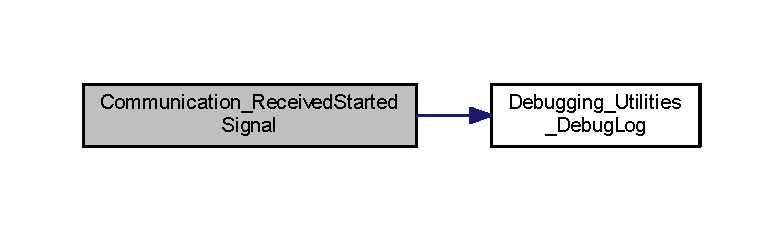
\includegraphics[width=350pt]{communication_8cpp_ab66ce78f3bfe62d6583da0a1a1473e6b_cgraph}
\end{center}
\end{figure}
Here is the caller graph for this function\+:\nopagebreak
\begin{figure}[H]
\begin{center}
\leavevmode
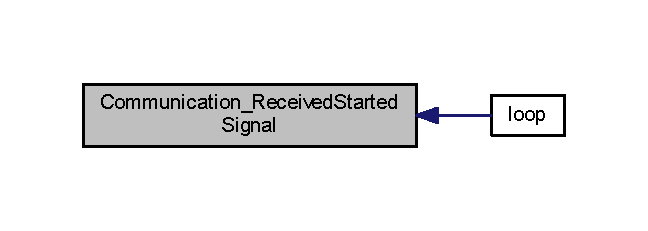
\includegraphics[width=311pt]{communication_8cpp_ab66ce78f3bfe62d6583da0a1a1473e6b_icgraph}
\end{center}
\end{figure}
\mbox{\Hypertarget{communication_8cpp_ab24ce0353afa549bb631933e8cfe9343}\label{communication_8cpp_ab24ce0353afa549bb631933e8cfe9343}} 
\index{communication.\+cpp@{communication.\+cpp}!Communication\+\_\+\+Received\+Stopped\+Signal@{Communication\+\_\+\+Received\+Stopped\+Signal}}
\index{Communication\+\_\+\+Received\+Stopped\+Signal@{Communication\+\_\+\+Received\+Stopped\+Signal}!communication.\+cpp@{communication.\+cpp}}
\subsubsection{\texorpdfstring{Communication\+\_\+\+Received\+Stopped\+Signal()}{Communication\_ReceivedStoppedSignal()}}
{\footnotesize\ttfamily void Communication\+\_\+\+Received\+Stopped\+Signal (\begin{DoxyParamCaption}{ }\end{DoxyParamCaption})}

Called when received Function ID \char`\"{}2\char`\"{}.

This function indicates to the ground station that the satellite has stoppped.

Received\+: satellite\textquotesingle{}s failure is detected.

\begin{DoxyRefDesc}{Todo}
\item[\mbox{\hyperlink{todo__todo000002}{Todo}}]Implement satellite stop signal transmission. \end{DoxyRefDesc}
Here is the call graph for this function\+:\nopagebreak
\begin{figure}[H]
\begin{center}
\leavevmode
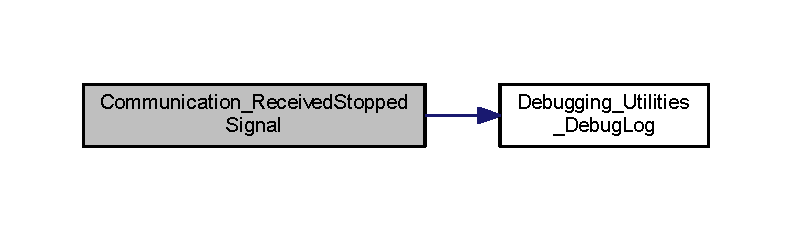
\includegraphics[width=350pt]{communication_8cpp_ab24ce0353afa549bb631933e8cfe9343_cgraph}
\end{center}
\end{figure}
Here is the caller graph for this function\+:\nopagebreak
\begin{figure}[H]
\begin{center}
\leavevmode
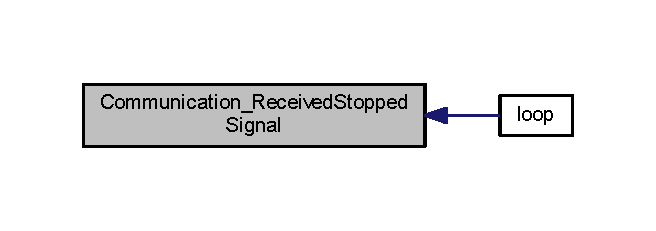
\includegraphics[width=315pt]{communication_8cpp_ab24ce0353afa549bb631933e8cfe9343_icgraph}
\end{center}
\end{figure}
\mbox{\Hypertarget{communication_8cpp_a18e4470849a0b104b638efb80f2f56d7}\label{communication_8cpp_a18e4470849a0b104b638efb80f2f56d7}} 
\index{communication.\+cpp@{communication.\+cpp}!Communication\+\_\+\+Received\+Transceiver\+Settings@{Communication\+\_\+\+Received\+Transceiver\+Settings}}
\index{Communication\+\_\+\+Received\+Transceiver\+Settings@{Communication\+\_\+\+Received\+Transceiver\+Settings}!communication.\+cpp@{communication.\+cpp}}
\subsubsection{\texorpdfstring{Communication\+\_\+\+Received\+Transceiver\+Settings()}{Communication\_ReceivedTransceiverSettings()}}
{\footnotesize\ttfamily void Communication\+\_\+\+Received\+Transceiver\+Settings (\begin{DoxyParamCaption}\item[{String}]{in\+Message,  }\item[{float}]{in\+Frequency\+Error }\end{DoxyParamCaption})}

Function ID \char`\"{}10\char`\"{}.

This function is called when the ground station receives a tranceiver setting transmission. This transmission tunes the ground station to the satellite.

This function\textquotesingle{}s associated transmission is sent from the satellite in a wide bandwidth (62.\+5\+K\+Hz) mode. Upon the ground station receiving this wide bandwidth transmission, it uses the frequency error (how much the default 434.\+0 M\+Hz frequency has been distorted) to re-\/set the frequency the ground stations S\+X1278 listen to.

After the ground station has tuned itself, it switches to a small bandwidth (7.\+8\+K\+Hz) mode. If the ground station cannot communicate with the satellite, or packets are failed to be sent, it switches back to the \char`\"{}searching\char`\"{} wide bandwidth mode.

If the ground station L\+O\+R\+A.\+receive() function returns a timeout, it resets to width bandwidth \char`\"{}searching/listening\char`\"{} mode for re-\/tuning.

Received\+: Every 1s from the satellite\textquotesingle{}s Loop(). Here is the call graph for this function\+:\nopagebreak
\begin{figure}[H]
\begin{center}
\leavevmode
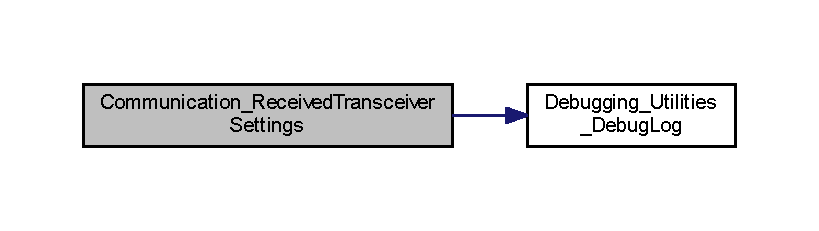
\includegraphics[width=350pt]{communication_8cpp_a18e4470849a0b104b638efb80f2f56d7_cgraph}
\end{center}
\end{figure}
Here is the caller graph for this function\+:\nopagebreak
\begin{figure}[H]
\begin{center}
\leavevmode
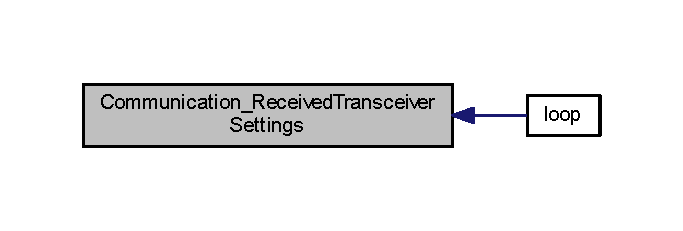
\includegraphics[width=328pt]{communication_8cpp_a18e4470849a0b104b638efb80f2f56d7_icgraph}
\end{center}
\end{figure}
\mbox{\Hypertarget{communication_8cpp_a9120f84592164d2c696fc5d8b9948ac1}\label{communication_8cpp_a9120f84592164d2c696fc5d8b9948ac1}} 
\index{communication.\+cpp@{communication.\+cpp}!Communication\+\_\+\+Received\+Transmitted\+Online@{Communication\+\_\+\+Received\+Transmitted\+Online}}
\index{Communication\+\_\+\+Received\+Transmitted\+Online@{Communication\+\_\+\+Received\+Transmitted\+Online}!communication.\+cpp@{communication.\+cpp}}
\subsubsection{\texorpdfstring{Communication\+\_\+\+Received\+Transmitted\+Online()}{Communication\_ReceivedTransmittedOnline()}}
{\footnotesize\ttfamily void Communication\+\_\+\+Received\+Transmitted\+Online (\begin{DoxyParamCaption}{ }\end{DoxyParamCaption})}

Called when received Function ID \char`\"{}2\char`\"{}.

This function indicates to the ground station that the satellite has initialised it\textquotesingle{}s transceiver.

Received\+: satellite\textquotesingle{}s failure is detected.

\begin{DoxyRefDesc}{Todo}
\item[\mbox{\hyperlink{todo__todo000003}{Todo}}]Add output interface. 

Implement satellite stop signal transmission.\end{DoxyRefDesc}
Here is the call graph for this function\+:\nopagebreak
\begin{figure}[H]
\begin{center}
\leavevmode
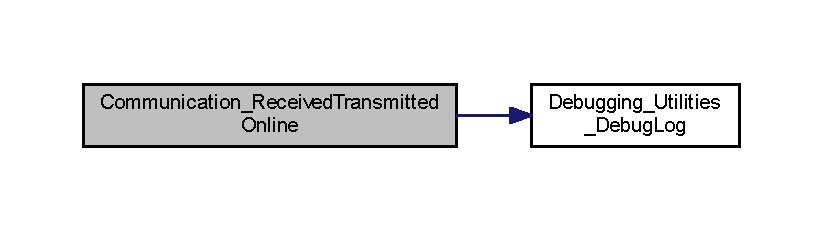
\includegraphics[width=350pt]{communication_8cpp_a9120f84592164d2c696fc5d8b9948ac1_cgraph}
\end{center}
\end{figure}
Here is the caller graph for this function\+:\nopagebreak
\begin{figure}[H]
\begin{center}
\leavevmode
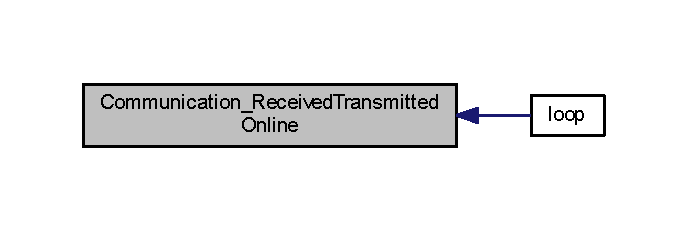
\includegraphics[width=330pt]{communication_8cpp_a9120f84592164d2c696fc5d8b9948ac1_icgraph}
\end{center}
\end{figure}
\mbox{\Hypertarget{communication_8cpp_a68fd88d1ccfc91925d30c0fdf1b417ab}\label{communication_8cpp_a68fd88d1ccfc91925d30c0fdf1b417ab}} 
\index{communication.\+cpp@{communication.\+cpp}!Communication\+\_\+\+S\+X1278\+Transmit@{Communication\+\_\+\+S\+X1278\+Transmit}}
\index{Communication\+\_\+\+S\+X1278\+Transmit@{Communication\+\_\+\+S\+X1278\+Transmit}!communication.\+cpp@{communication.\+cpp}}
\subsubsection{\texorpdfstring{Communication\+\_\+\+S\+X1278\+Transmit()}{Communication\_SX1278Transmit()}}
{\footnotesize\ttfamily void Communication\+\_\+\+S\+X1278\+Transmit (\begin{DoxyParamCaption}\item[{String}]{in\+Func\+Id,  }\item[{String}]{in\+Message }\end{DoxyParamCaption})}

The main transmission function. 
\begin{DoxyParams}{Parameters}
{\em in\+Func\+Id} & The number that represents the function being sent. \\
\hline
{\em in\+Message} & The string that will be transmistted to the satellite.\\
\hline
\end{DoxyParams}
This should never be called directly in the main code body. There are more specific functions that handle custom functionality.

\begin{DoxyRefDesc}{Todo}
\item[\mbox{\hyperlink{todo__todo000001}{Todo}}]Debug Logging removal. 

Transmission signature containment. \end{DoxyRefDesc}
\begin{DoxyRefDesc}{Test}
\item[\mbox{\hyperlink{test__test000001}{Test}}]in\+Func\+Id range String(-\/inf) to String(inf). 

in\+Func\+Id String length above 256 

In\+Func\+Id empty string. 

in\+Message String empty. 

in\+Message length above 256. \end{DoxyRefDesc}
Here is the call graph for this function\+:\nopagebreak
\begin{figure}[H]
\begin{center}
\leavevmode
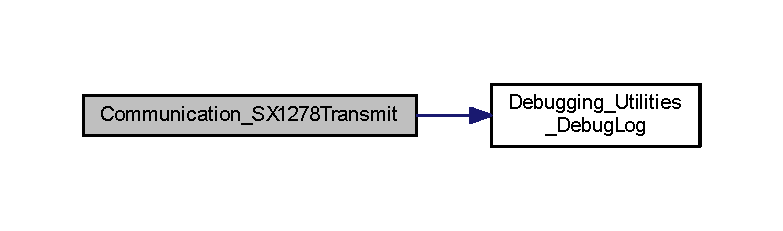
\includegraphics[width=350pt]{communication_8cpp_a68fd88d1ccfc91925d30c0fdf1b417ab_cgraph}
\end{center}
\end{figure}
Here is the caller graph for this function\+:\nopagebreak
\begin{figure}[H]
\begin{center}
\leavevmode
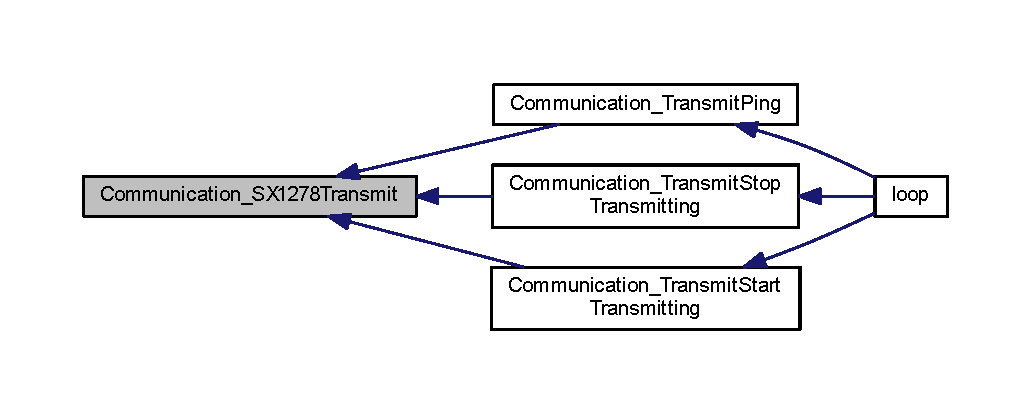
\includegraphics[width=350pt]{communication_8cpp_a68fd88d1ccfc91925d30c0fdf1b417ab_icgraph}
\end{center}
\end{figure}
\mbox{\Hypertarget{communication_8cpp_a639d7624642ba6e8f368f15b89d1b557}\label{communication_8cpp_a639d7624642ba6e8f368f15b89d1b557}} 
\index{communication.\+cpp@{communication.\+cpp}!Communication\+\_\+\+Transmit\+Ping@{Communication\+\_\+\+Transmit\+Ping}}
\index{Communication\+\_\+\+Transmit\+Ping@{Communication\+\_\+\+Transmit\+Ping}!communication.\+cpp@{communication.\+cpp}}
\subsubsection{\texorpdfstring{Communication\+\_\+\+Transmit\+Ping()}{Communication\_TransmitPing()}}
{\footnotesize\ttfamily void Communication\+\_\+\+Transmit\+Ping (\begin{DoxyParamCaption}{ }\end{DoxyParamCaption})}

Function ID \char`\"{}5\char`\"{}.

This function transmits to the satellite a small packet, the satellite then responds with a Pong packet. This is useful for small packet testing the connection.

Transmitted\+: On user input.

\begin{DoxyRefDesc}{Todo}
\item[\mbox{\hyperlink{todo__todo000005}{Todo}}]Implement user interface for ground station. \end{DoxyRefDesc}
Here is the call graph for this function\+:\nopagebreak
\begin{figure}[H]
\begin{center}
\leavevmode
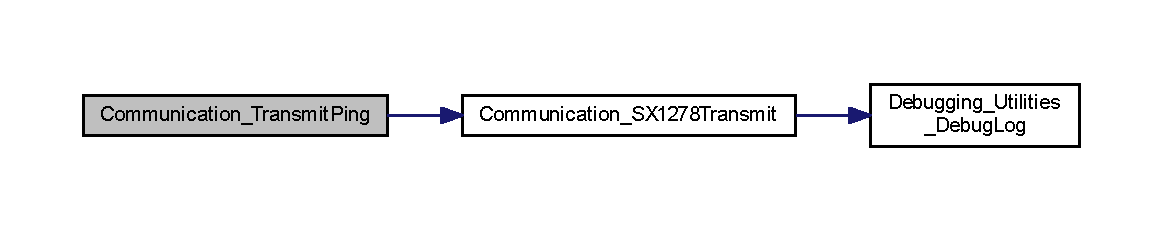
\includegraphics[width=350pt]{communication_8cpp_a639d7624642ba6e8f368f15b89d1b557_cgraph}
\end{center}
\end{figure}
Here is the caller graph for this function\+:\nopagebreak
\begin{figure}[H]
\begin{center}
\leavevmode
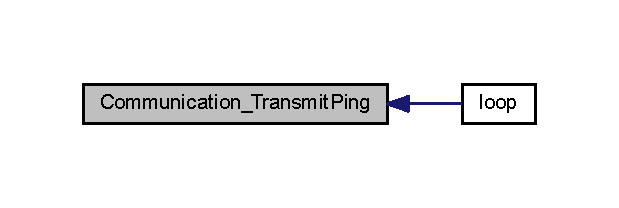
\includegraphics[width=297pt]{communication_8cpp_a639d7624642ba6e8f368f15b89d1b557_icgraph}
\end{center}
\end{figure}
\mbox{\Hypertarget{communication_8cpp_aa11cefca5402f3a480be0b8448916dab}\label{communication_8cpp_aa11cefca5402f3a480be0b8448916dab}} 
\index{communication.\+cpp@{communication.\+cpp}!Communication\+\_\+\+Transmit\+Start\+Transmitting@{Communication\+\_\+\+Transmit\+Start\+Transmitting}}
\index{Communication\+\_\+\+Transmit\+Start\+Transmitting@{Communication\+\_\+\+Transmit\+Start\+Transmitting}!communication.\+cpp@{communication.\+cpp}}
\subsubsection{\texorpdfstring{Communication\+\_\+\+Transmit\+Start\+Transmitting()}{Communication\_TransmitStartTransmitting()}}
{\footnotesize\ttfamily void Communication\+\_\+\+Transmit\+Start\+Transmitting (\begin{DoxyParamCaption}{ }\end{DoxyParamCaption})}

Function ID \char`\"{}8\char`\"{}.

This function signals to the satellite to start transmitting again. When the satellite is given a \char`\"{}\+Stop Transmitting\char`\"{} signal it will only listen for this signal and nothing else.

Transmitted\+: On user input.

\begin{DoxyRefDesc}{Todo}
\item[\mbox{\hyperlink{todo__todo000007}{Todo}}]Reference the security code that requires this functionality. \end{DoxyRefDesc}
Here is the call graph for this function\+:\nopagebreak
\begin{figure}[H]
\begin{center}
\leavevmode
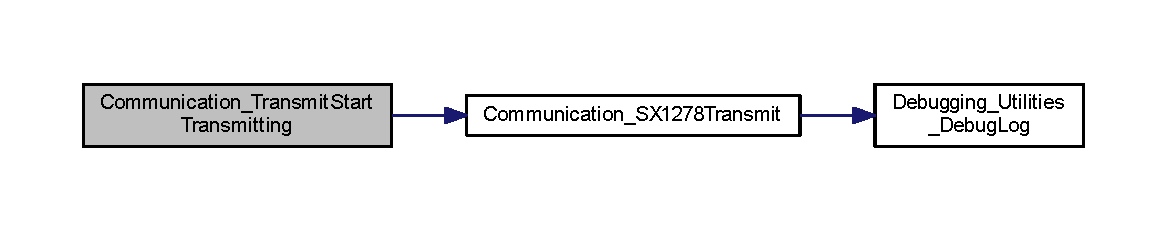
\includegraphics[width=350pt]{communication_8cpp_aa11cefca5402f3a480be0b8448916dab_cgraph}
\end{center}
\end{figure}
Here is the caller graph for this function\+:\nopagebreak
\begin{figure}[H]
\begin{center}
\leavevmode
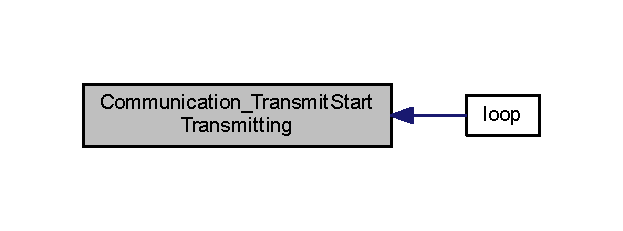
\includegraphics[width=299pt]{communication_8cpp_aa11cefca5402f3a480be0b8448916dab_icgraph}
\end{center}
\end{figure}
\mbox{\Hypertarget{communication_8cpp_a7d368a63e53f4a1a63b166e6e97c7805}\label{communication_8cpp_a7d368a63e53f4a1a63b166e6e97c7805}} 
\index{communication.\+cpp@{communication.\+cpp}!Communication\+\_\+\+Transmit\+Stop\+Transmitting@{Communication\+\_\+\+Transmit\+Stop\+Transmitting}}
\index{Communication\+\_\+\+Transmit\+Stop\+Transmitting@{Communication\+\_\+\+Transmit\+Stop\+Transmitting}!communication.\+cpp@{communication.\+cpp}}
\subsubsection{\texorpdfstring{Communication\+\_\+\+Transmit\+Stop\+Transmitting()}{Communication\_TransmitStopTransmitting()}}
{\footnotesize\ttfamily void Communication\+\_\+\+Transmit\+Stop\+Transmitting (\begin{DoxyParamCaption}{ }\end{DoxyParamCaption})}

Function ID \char`\"{}7\char`\"{}.

This function signals to the satellite to stop all transmissions.

Transmitted\+: On user input.

\begin{DoxyRefDesc}{Todo}
\item[\mbox{\hyperlink{todo__todo000006}{Todo}}]Reference the security code that requires this functionality. \end{DoxyRefDesc}
Here is the call graph for this function\+:\nopagebreak
\begin{figure}[H]
\begin{center}
\leavevmode
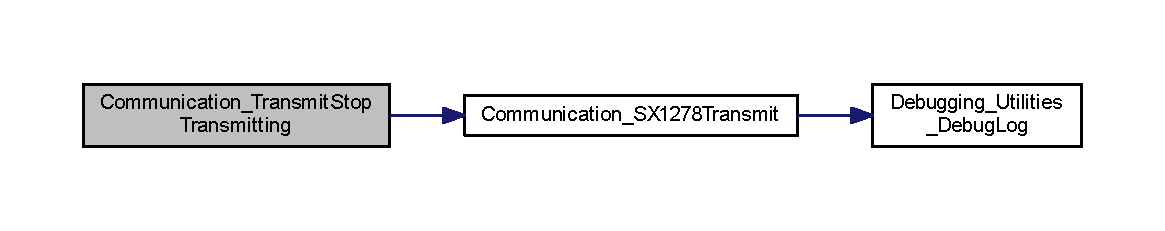
\includegraphics[width=350pt]{communication_8cpp_a7d368a63e53f4a1a63b166e6e97c7805_cgraph}
\end{center}
\end{figure}
Here is the caller graph for this function\+:\nopagebreak
\begin{figure}[H]
\begin{center}
\leavevmode
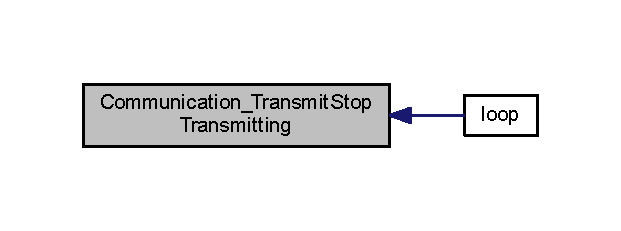
\includegraphics[width=298pt]{communication_8cpp_a7d368a63e53f4a1a63b166e6e97c7805_icgraph}
\end{center}
\end{figure}

\hypertarget{communication_8h}{}\section{communication.\+h File Reference}
\label{communication_8h}\index{communication.\+h@{communication.\+h}}
This graph shows which files directly or indirectly include this file\+:\nopagebreak
\begin{figure}[H]
\begin{center}
\leavevmode
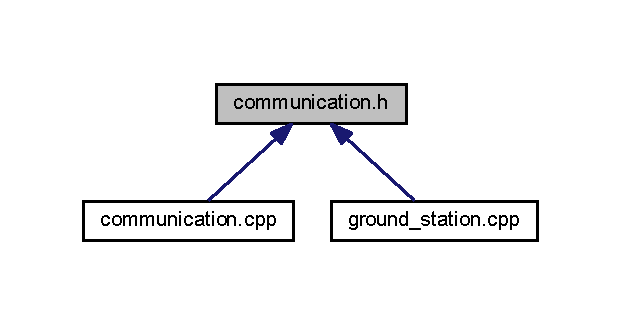
\includegraphics[width=298pt]{communication_8h__dep__incl}
\end{center}
\end{figure}
\subsection*{Functions}
\begin{DoxyCompactItemize}
\item 
void \mbox{\hyperlink{communication_8h_a68fd88d1ccfc91925d30c0fdf1b417ab}{Communication\+\_\+\+S\+X1278\+Transmit}} (String in\+Func\+Id, String in\+Message)
\item 
void \mbox{\hyperlink{communication_8h_ab66ce78f3bfe62d6583da0a1a1473e6b}{Communication\+\_\+\+Received\+Started\+Signal}} ()
\item 
void \mbox{\hyperlink{communication_8h_ab24ce0353afa549bb631933e8cfe9343}{Communication\+\_\+\+Received\+Stopped\+Signal}} ()
\item 
void \mbox{\hyperlink{communication_8h_a9120f84592164d2c696fc5d8b9948ac1}{Communication\+\_\+\+Received\+Transmitted\+Online}} ()
\item 
void \mbox{\hyperlink{communication_8h_a649fe6cc16cc68a0eda736de6d670ea4}{Communication\+\_\+\+Received\+Deployment\+Success}} ()
\item 
void \mbox{\hyperlink{communication_8h_a639d7624642ba6e8f368f15b89d1b557}{Communication\+\_\+\+Transmit\+Ping}} ()
\item 
void \mbox{\hyperlink{communication_8h_a7d368a63e53f4a1a63b166e6e97c7805}{Communication\+\_\+\+Transmit\+Stop\+Transmitting}} ()
\item 
void \mbox{\hyperlink{communication_8h_aa11cefca5402f3a480be0b8448916dab}{Communication\+\_\+\+Transmit\+Start\+Transmitting}} ()
\item 
void \mbox{\hyperlink{communication_8h_a9dd32118d0d9d6eaa0cf4c5646622549}{Communication\+\_\+\+Received\+Power\+Info}} (String in\+Message)
\item 
void \mbox{\hyperlink{communication_8h_ad67fe0fd5088334be55f2045f5c2067f}{Communication\+\_\+\+Received\+Pong}} ()
\item 
void \mbox{\hyperlink{communication_8h_a18e4470849a0b104b638efb80f2f56d7}{Communication\+\_\+\+Received\+Transceiver\+Settings}} (String in\+Message, float in\+Frequency\+Error)
\end{DoxyCompactItemize}


\subsection{Function Documentation}
\mbox{\Hypertarget{communication_8h_a649fe6cc16cc68a0eda736de6d670ea4}\label{communication_8h_a649fe6cc16cc68a0eda736de6d670ea4}} 
\index{communication.\+h@{communication.\+h}!Communication\+\_\+\+Received\+Deployment\+Success@{Communication\+\_\+\+Received\+Deployment\+Success}}
\index{Communication\+\_\+\+Received\+Deployment\+Success@{Communication\+\_\+\+Received\+Deployment\+Success}!communication.\+h@{communication.\+h}}
\subsubsection{\texorpdfstring{Communication\+\_\+\+Received\+Deployment\+Success()}{Communication\_ReceivedDeploymentSuccess()}}
{\footnotesize\ttfamily void Communication\+\_\+\+Received\+Deployment\+Success (\begin{DoxyParamCaption}{ }\end{DoxyParamCaption})}

Called when received Function ID \char`\"{}4\char`\"{}.

This function indicates to the ground station that the deployment sequence was successfull.

Received\+: Satellite\textquotesingle{}s Setup() function.

\begin{DoxyRefDesc}{Todo}
\item[\mbox{\hyperlink{todo__todo000004}{Todo}}]Implement satellite deployment success signal. \end{DoxyRefDesc}
Here is the call graph for this function\+:\nopagebreak
\begin{figure}[H]
\begin{center}
\leavevmode
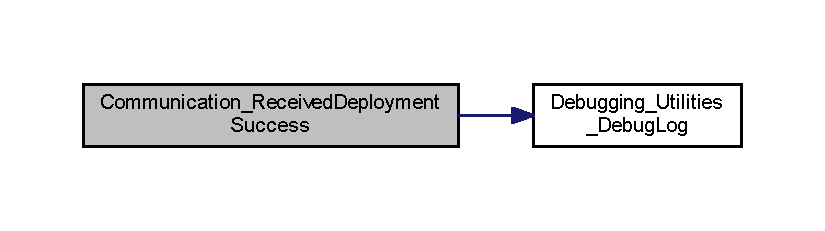
\includegraphics[width=350pt]{communication_8h_a649fe6cc16cc68a0eda736de6d670ea4_cgraph}
\end{center}
\end{figure}
Here is the caller graph for this function\+:\nopagebreak
\begin{figure}[H]
\begin{center}
\leavevmode
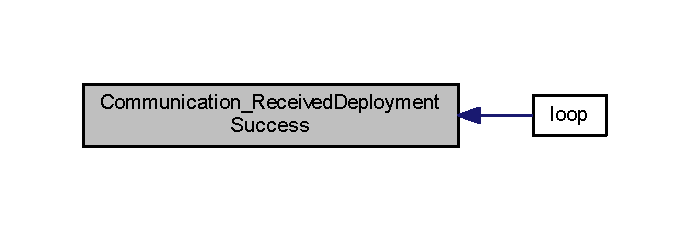
\includegraphics[width=331pt]{communication_8h_a649fe6cc16cc68a0eda736de6d670ea4_icgraph}
\end{center}
\end{figure}
\mbox{\Hypertarget{communication_8h_ad67fe0fd5088334be55f2045f5c2067f}\label{communication_8h_ad67fe0fd5088334be55f2045f5c2067f}} 
\index{communication.\+h@{communication.\+h}!Communication\+\_\+\+Received\+Pong@{Communication\+\_\+\+Received\+Pong}}
\index{Communication\+\_\+\+Received\+Pong@{Communication\+\_\+\+Received\+Pong}!communication.\+h@{communication.\+h}}
\subsubsection{\texorpdfstring{Communication\+\_\+\+Received\+Pong()}{Communication\_ReceivedPong()}}
{\footnotesize\ttfamily void Communication\+\_\+\+Received\+Pong (\begin{DoxyParamCaption}{ }\end{DoxyParamCaption})}

Called when received Function ID \char`\"{}6\char`\"{}.

This function indicates to the ground station that the satellite received the Ping transmission.

Received\+: Satellite receives Ping function \char`\"{}5\char`\"{} transmission. Here is the call graph for this function\+:\nopagebreak
\begin{figure}[H]
\begin{center}
\leavevmode
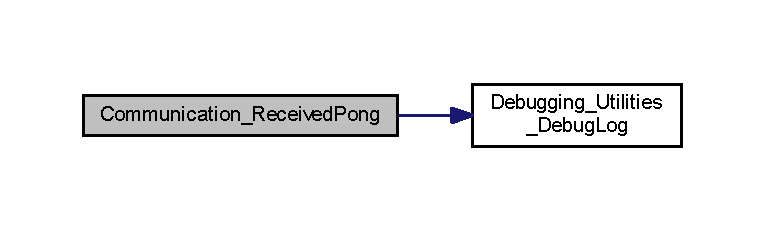
\includegraphics[width=350pt]{communication_8h_ad67fe0fd5088334be55f2045f5c2067f_cgraph}
\end{center}
\end{figure}
Here is the caller graph for this function\+:\nopagebreak
\begin{figure}[H]
\begin{center}
\leavevmode
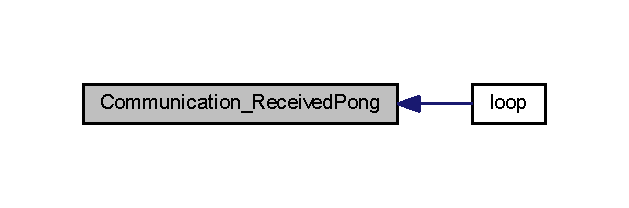
\includegraphics[width=302pt]{communication_8h_ad67fe0fd5088334be55f2045f5c2067f_icgraph}
\end{center}
\end{figure}
\mbox{\Hypertarget{communication_8h_a9dd32118d0d9d6eaa0cf4c5646622549}\label{communication_8h_a9dd32118d0d9d6eaa0cf4c5646622549}} 
\index{communication.\+h@{communication.\+h}!Communication\+\_\+\+Received\+Power\+Info@{Communication\+\_\+\+Received\+Power\+Info}}
\index{Communication\+\_\+\+Received\+Power\+Info@{Communication\+\_\+\+Received\+Power\+Info}!communication.\+h@{communication.\+h}}
\subsubsection{\texorpdfstring{Communication\+\_\+\+Received\+Power\+Info()}{Communication\_ReceivedPowerInfo()}}
{\footnotesize\ttfamily void Communication\+\_\+\+Received\+Power\+Info (\begin{DoxyParamCaption}\item[{String}]{in\+Message }\end{DoxyParamCaption})}

Function ID \char`\"{}9\char`\"{}.

This function is called when the ground station receives a power infomation transmission. The power info is broadcasted every 400s.

Received\+: every 400ms from the satellite\textquotesingle{}s Loop(). Here is the call graph for this function\+:\nopagebreak
\begin{figure}[H]
\begin{center}
\leavevmode
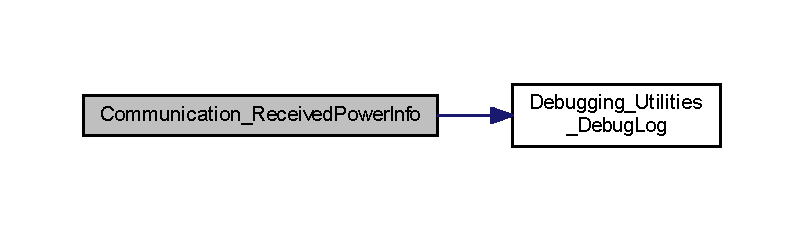
\includegraphics[width=350pt]{communication_8h_a9dd32118d0d9d6eaa0cf4c5646622549_cgraph}
\end{center}
\end{figure}
Here is the caller graph for this function\+:\nopagebreak
\begin{figure}[H]
\begin{center}
\leavevmode
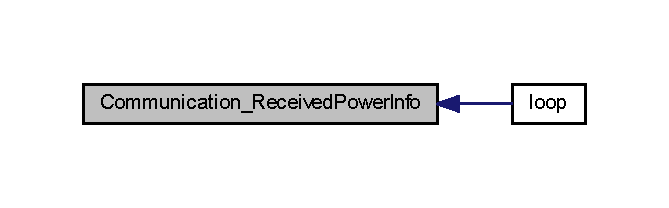
\includegraphics[width=321pt]{communication_8h_a9dd32118d0d9d6eaa0cf4c5646622549_icgraph}
\end{center}
\end{figure}
\mbox{\Hypertarget{communication_8h_ab66ce78f3bfe62d6583da0a1a1473e6b}\label{communication_8h_ab66ce78f3bfe62d6583da0a1a1473e6b}} 
\index{communication.\+h@{communication.\+h}!Communication\+\_\+\+Received\+Started\+Signal@{Communication\+\_\+\+Received\+Started\+Signal}}
\index{Communication\+\_\+\+Received\+Started\+Signal@{Communication\+\_\+\+Received\+Started\+Signal}!communication.\+h@{communication.\+h}}
\subsubsection{\texorpdfstring{Communication\+\_\+\+Received\+Started\+Signal()}{Communication\_ReceivedStartedSignal()}}
{\footnotesize\ttfamily void Communication\+\_\+\+Received\+Started\+Signal (\begin{DoxyParamCaption}{ }\end{DoxyParamCaption})}

Called when received Function ID \char`\"{}1\char`\"{}.

This function indicates to the ground station that the satellite has started.

Received\+: satellite\textquotesingle{}s Setup() function is called.. Here is the call graph for this function\+:\nopagebreak
\begin{figure}[H]
\begin{center}
\leavevmode
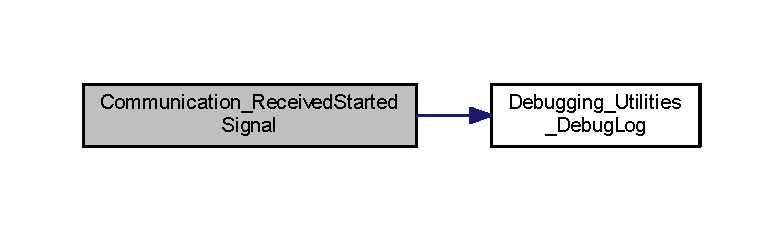
\includegraphics[width=350pt]{communication_8h_ab66ce78f3bfe62d6583da0a1a1473e6b_cgraph}
\end{center}
\end{figure}
Here is the caller graph for this function\+:\nopagebreak
\begin{figure}[H]
\begin{center}
\leavevmode
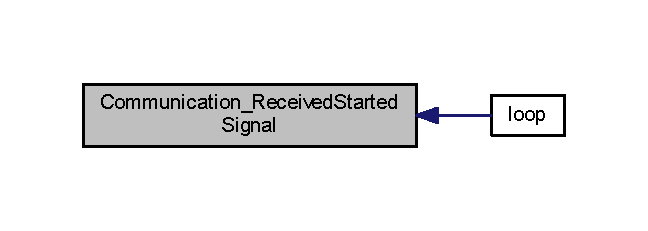
\includegraphics[width=311pt]{communication_8h_ab66ce78f3bfe62d6583da0a1a1473e6b_icgraph}
\end{center}
\end{figure}
\mbox{\Hypertarget{communication_8h_ab24ce0353afa549bb631933e8cfe9343}\label{communication_8h_ab24ce0353afa549bb631933e8cfe9343}} 
\index{communication.\+h@{communication.\+h}!Communication\+\_\+\+Received\+Stopped\+Signal@{Communication\+\_\+\+Received\+Stopped\+Signal}}
\index{Communication\+\_\+\+Received\+Stopped\+Signal@{Communication\+\_\+\+Received\+Stopped\+Signal}!communication.\+h@{communication.\+h}}
\subsubsection{\texorpdfstring{Communication\+\_\+\+Received\+Stopped\+Signal()}{Communication\_ReceivedStoppedSignal()}}
{\footnotesize\ttfamily void Communication\+\_\+\+Received\+Stopped\+Signal (\begin{DoxyParamCaption}{ }\end{DoxyParamCaption})}

Called when received Function ID \char`\"{}2\char`\"{}.

This function indicates to the ground station that the satellite has stoppped.

Received\+: satellite\textquotesingle{}s failure is detected.

\begin{DoxyRefDesc}{Todo}
\item[\mbox{\hyperlink{todo__todo000002}{Todo}}]Implement satellite stop signal transmission. \end{DoxyRefDesc}
Here is the call graph for this function\+:\nopagebreak
\begin{figure}[H]
\begin{center}
\leavevmode
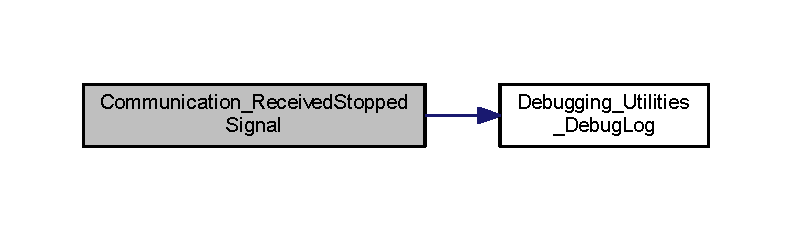
\includegraphics[width=350pt]{communication_8h_ab24ce0353afa549bb631933e8cfe9343_cgraph}
\end{center}
\end{figure}
Here is the caller graph for this function\+:\nopagebreak
\begin{figure}[H]
\begin{center}
\leavevmode
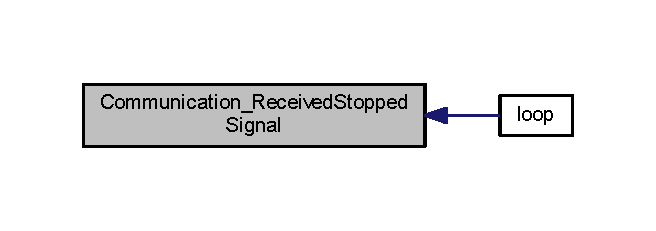
\includegraphics[width=315pt]{communication_8h_ab24ce0353afa549bb631933e8cfe9343_icgraph}
\end{center}
\end{figure}
\mbox{\Hypertarget{communication_8h_a18e4470849a0b104b638efb80f2f56d7}\label{communication_8h_a18e4470849a0b104b638efb80f2f56d7}} 
\index{communication.\+h@{communication.\+h}!Communication\+\_\+\+Received\+Transceiver\+Settings@{Communication\+\_\+\+Received\+Transceiver\+Settings}}
\index{Communication\+\_\+\+Received\+Transceiver\+Settings@{Communication\+\_\+\+Received\+Transceiver\+Settings}!communication.\+h@{communication.\+h}}
\subsubsection{\texorpdfstring{Communication\+\_\+\+Received\+Transceiver\+Settings()}{Communication\_ReceivedTransceiverSettings()}}
{\footnotesize\ttfamily void Communication\+\_\+\+Received\+Transceiver\+Settings (\begin{DoxyParamCaption}\item[{String}]{in\+Message,  }\item[{float}]{in\+Frequency\+Error }\end{DoxyParamCaption})}

Function ID \char`\"{}10\char`\"{}.

This function is called when the ground station receives a tranceiver setting transmission. This transmission tunes the ground station to the satellite.

This function\textquotesingle{}s associated transmission is sent from the satellite in a wide bandwidth (62.\+5\+K\+Hz) mode. Upon the ground station receiving this wide bandwidth transmission, it uses the frequency error (how much the default 434.\+0 M\+Hz frequency has been distorted) to re-\/set the frequency the ground stations S\+X1278 listen to.

After the ground station has tuned itself, it switches to a small bandwidth (7.\+8\+K\+Hz) mode. If the ground station cannot communicate with the satellite, or packets are failed to be sent, it switches back to the \char`\"{}searching\char`\"{} wide bandwidth mode.

If the ground station L\+O\+R\+A.\+receive() function returns a timeout, it resets to width bandwidth \char`\"{}searching/listening\char`\"{} mode for re-\/tuning.

Received\+: Every 1s from the satellite\textquotesingle{}s Loop(). Here is the call graph for this function\+:\nopagebreak
\begin{figure}[H]
\begin{center}
\leavevmode
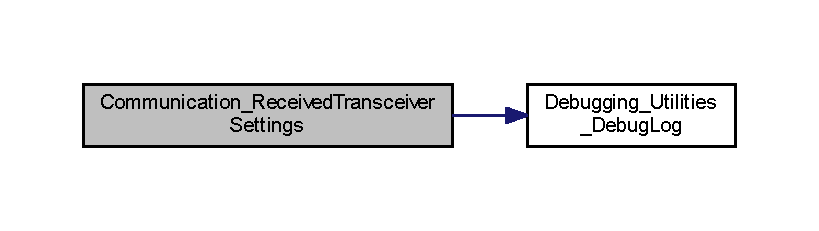
\includegraphics[width=350pt]{communication_8h_a18e4470849a0b104b638efb80f2f56d7_cgraph}
\end{center}
\end{figure}
Here is the caller graph for this function\+:\nopagebreak
\begin{figure}[H]
\begin{center}
\leavevmode
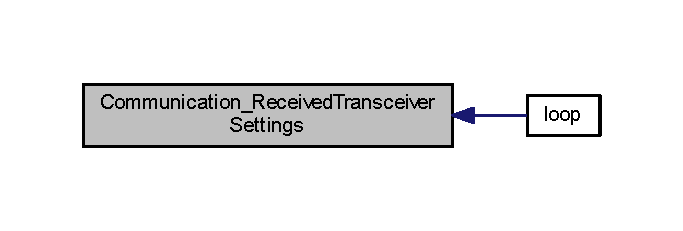
\includegraphics[width=328pt]{communication_8h_a18e4470849a0b104b638efb80f2f56d7_icgraph}
\end{center}
\end{figure}
\mbox{\Hypertarget{communication_8h_a9120f84592164d2c696fc5d8b9948ac1}\label{communication_8h_a9120f84592164d2c696fc5d8b9948ac1}} 
\index{communication.\+h@{communication.\+h}!Communication\+\_\+\+Received\+Transmitted\+Online@{Communication\+\_\+\+Received\+Transmitted\+Online}}
\index{Communication\+\_\+\+Received\+Transmitted\+Online@{Communication\+\_\+\+Received\+Transmitted\+Online}!communication.\+h@{communication.\+h}}
\subsubsection{\texorpdfstring{Communication\+\_\+\+Received\+Transmitted\+Online()}{Communication\_ReceivedTransmittedOnline()}}
{\footnotesize\ttfamily void Communication\+\_\+\+Received\+Transmitted\+Online (\begin{DoxyParamCaption}{ }\end{DoxyParamCaption})}

Called when received Function ID \char`\"{}2\char`\"{}.

This function indicates to the ground station that the satellite has initialised it\textquotesingle{}s transceiver.

Received\+: satellite\textquotesingle{}s failure is detected.

\begin{DoxyRefDesc}{Todo}
\item[\mbox{\hyperlink{todo__todo000003}{Todo}}]Add output interface. 

Implement satellite stop signal transmission.\end{DoxyRefDesc}
Here is the call graph for this function\+:\nopagebreak
\begin{figure}[H]
\begin{center}
\leavevmode
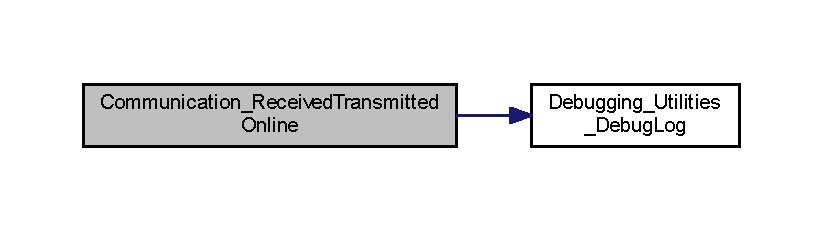
\includegraphics[width=350pt]{communication_8h_a9120f84592164d2c696fc5d8b9948ac1_cgraph}
\end{center}
\end{figure}
Here is the caller graph for this function\+:\nopagebreak
\begin{figure}[H]
\begin{center}
\leavevmode
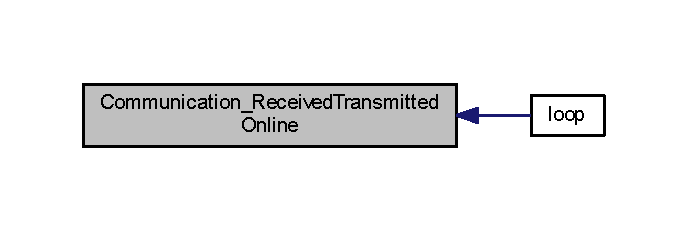
\includegraphics[width=330pt]{communication_8h_a9120f84592164d2c696fc5d8b9948ac1_icgraph}
\end{center}
\end{figure}
\mbox{\Hypertarget{communication_8h_a68fd88d1ccfc91925d30c0fdf1b417ab}\label{communication_8h_a68fd88d1ccfc91925d30c0fdf1b417ab}} 
\index{communication.\+h@{communication.\+h}!Communication\+\_\+\+S\+X1278\+Transmit@{Communication\+\_\+\+S\+X1278\+Transmit}}
\index{Communication\+\_\+\+S\+X1278\+Transmit@{Communication\+\_\+\+S\+X1278\+Transmit}!communication.\+h@{communication.\+h}}
\subsubsection{\texorpdfstring{Communication\+\_\+\+S\+X1278\+Transmit()}{Communication\_SX1278Transmit()}}
{\footnotesize\ttfamily void Communication\+\_\+\+S\+X1278\+Transmit (\begin{DoxyParamCaption}\item[{String}]{in\+Func\+Id,  }\item[{String}]{in\+Message }\end{DoxyParamCaption})}

The main transmission function. 
\begin{DoxyParams}{Parameters}
{\em in\+Func\+Id} & The number that represents the function being sent. \\
\hline
{\em in\+Message} & The string that will be transmistted to the satellite.\\
\hline
\end{DoxyParams}
This should never be called directly in the main code body. There are more specific functions that handle custom functionality.

\begin{DoxyRefDesc}{Todo}
\item[\mbox{\hyperlink{todo__todo000001}{Todo}}]Debug Logging removal. 

Transmission signature containment. \end{DoxyRefDesc}
\begin{DoxyRefDesc}{Test}
\item[\mbox{\hyperlink{test__test000001}{Test}}]in\+Func\+Id range String(-\/inf) to String(inf). 

in\+Func\+Id String length above 256 

In\+Func\+Id empty string. 

in\+Message String empty. 

in\+Message length above 256. \end{DoxyRefDesc}
Here is the call graph for this function\+:\nopagebreak
\begin{figure}[H]
\begin{center}
\leavevmode
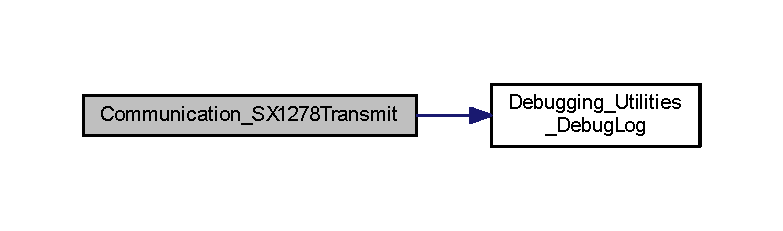
\includegraphics[width=350pt]{communication_8h_a68fd88d1ccfc91925d30c0fdf1b417ab_cgraph}
\end{center}
\end{figure}
Here is the caller graph for this function\+:\nopagebreak
\begin{figure}[H]
\begin{center}
\leavevmode
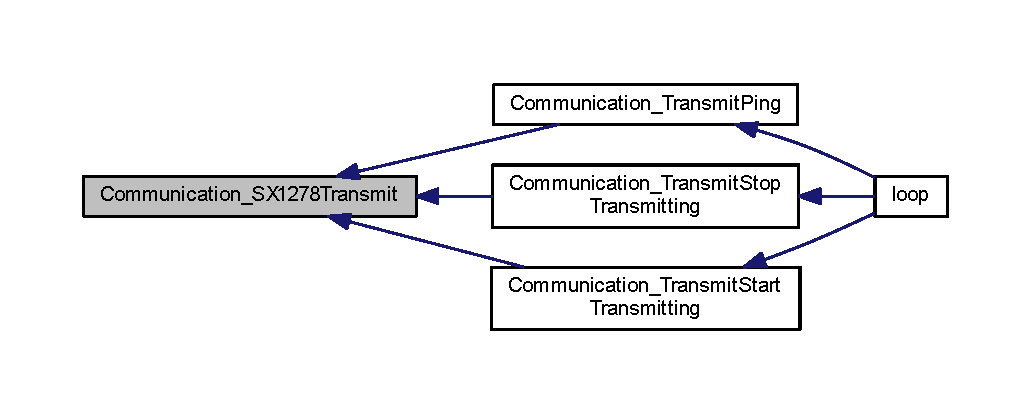
\includegraphics[width=350pt]{communication_8h_a68fd88d1ccfc91925d30c0fdf1b417ab_icgraph}
\end{center}
\end{figure}
\mbox{\Hypertarget{communication_8h_a639d7624642ba6e8f368f15b89d1b557}\label{communication_8h_a639d7624642ba6e8f368f15b89d1b557}} 
\index{communication.\+h@{communication.\+h}!Communication\+\_\+\+Transmit\+Ping@{Communication\+\_\+\+Transmit\+Ping}}
\index{Communication\+\_\+\+Transmit\+Ping@{Communication\+\_\+\+Transmit\+Ping}!communication.\+h@{communication.\+h}}
\subsubsection{\texorpdfstring{Communication\+\_\+\+Transmit\+Ping()}{Communication\_TransmitPing()}}
{\footnotesize\ttfamily void Communication\+\_\+\+Transmit\+Ping (\begin{DoxyParamCaption}{ }\end{DoxyParamCaption})}

Function ID \char`\"{}5\char`\"{}.

This function transmits to the satellite a small packet, the satellite then responds with a Pong packet. This is useful for small packet testing the connection.

Transmitted\+: On user input.

\begin{DoxyRefDesc}{Todo}
\item[\mbox{\hyperlink{todo__todo000005}{Todo}}]Implement user interface for ground station. \end{DoxyRefDesc}
Here is the call graph for this function\+:\nopagebreak
\begin{figure}[H]
\begin{center}
\leavevmode
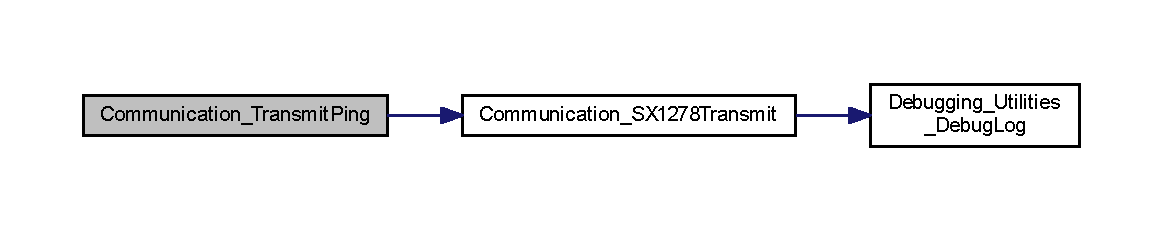
\includegraphics[width=350pt]{communication_8h_a639d7624642ba6e8f368f15b89d1b557_cgraph}
\end{center}
\end{figure}
Here is the caller graph for this function\+:\nopagebreak
\begin{figure}[H]
\begin{center}
\leavevmode
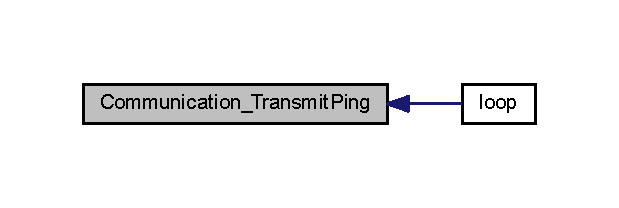
\includegraphics[width=297pt]{communication_8h_a639d7624642ba6e8f368f15b89d1b557_icgraph}
\end{center}
\end{figure}
\mbox{\Hypertarget{communication_8h_aa11cefca5402f3a480be0b8448916dab}\label{communication_8h_aa11cefca5402f3a480be0b8448916dab}} 
\index{communication.\+h@{communication.\+h}!Communication\+\_\+\+Transmit\+Start\+Transmitting@{Communication\+\_\+\+Transmit\+Start\+Transmitting}}
\index{Communication\+\_\+\+Transmit\+Start\+Transmitting@{Communication\+\_\+\+Transmit\+Start\+Transmitting}!communication.\+h@{communication.\+h}}
\subsubsection{\texorpdfstring{Communication\+\_\+\+Transmit\+Start\+Transmitting()}{Communication\_TransmitStartTransmitting()}}
{\footnotesize\ttfamily void Communication\+\_\+\+Transmit\+Start\+Transmitting (\begin{DoxyParamCaption}{ }\end{DoxyParamCaption})}

Function ID \char`\"{}8\char`\"{}.

This function signals to the satellite to start transmitting again. When the satellite is given a \char`\"{}\+Stop Transmitting\char`\"{} signal it will only listen for this signal and nothing else.

Transmitted\+: On user input.

\begin{DoxyRefDesc}{Todo}
\item[\mbox{\hyperlink{todo__todo000007}{Todo}}]Reference the security code that requires this functionality. \end{DoxyRefDesc}
Here is the call graph for this function\+:\nopagebreak
\begin{figure}[H]
\begin{center}
\leavevmode
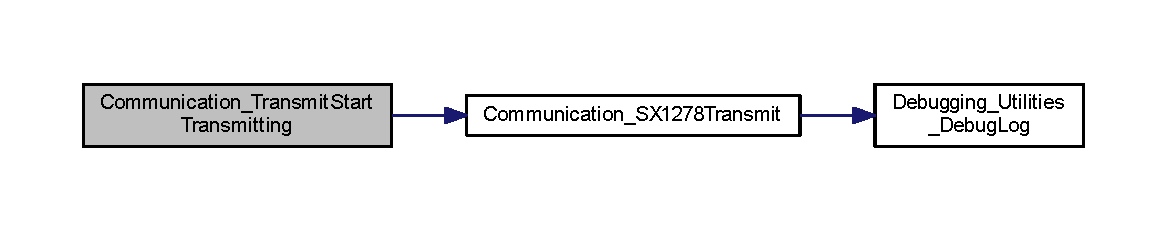
\includegraphics[width=350pt]{communication_8h_aa11cefca5402f3a480be0b8448916dab_cgraph}
\end{center}
\end{figure}
Here is the caller graph for this function\+:\nopagebreak
\begin{figure}[H]
\begin{center}
\leavevmode
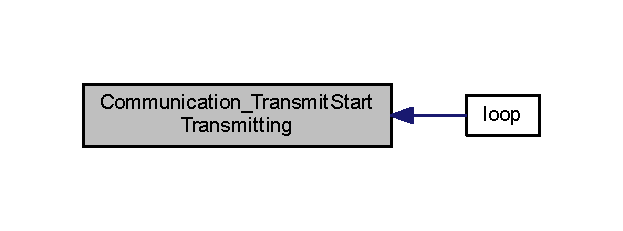
\includegraphics[width=299pt]{communication_8h_aa11cefca5402f3a480be0b8448916dab_icgraph}
\end{center}
\end{figure}
\mbox{\Hypertarget{communication_8h_a7d368a63e53f4a1a63b166e6e97c7805}\label{communication_8h_a7d368a63e53f4a1a63b166e6e97c7805}} 
\index{communication.\+h@{communication.\+h}!Communication\+\_\+\+Transmit\+Stop\+Transmitting@{Communication\+\_\+\+Transmit\+Stop\+Transmitting}}
\index{Communication\+\_\+\+Transmit\+Stop\+Transmitting@{Communication\+\_\+\+Transmit\+Stop\+Transmitting}!communication.\+h@{communication.\+h}}
\subsubsection{\texorpdfstring{Communication\+\_\+\+Transmit\+Stop\+Transmitting()}{Communication\_TransmitStopTransmitting()}}
{\footnotesize\ttfamily void Communication\+\_\+\+Transmit\+Stop\+Transmitting (\begin{DoxyParamCaption}{ }\end{DoxyParamCaption})}

Function ID \char`\"{}7\char`\"{}.

This function signals to the satellite to stop all transmissions.

Transmitted\+: On user input.

\begin{DoxyRefDesc}{Todo}
\item[\mbox{\hyperlink{todo__todo000006}{Todo}}]Reference the security code that requires this functionality. \end{DoxyRefDesc}
Here is the call graph for this function\+:\nopagebreak
\begin{figure}[H]
\begin{center}
\leavevmode
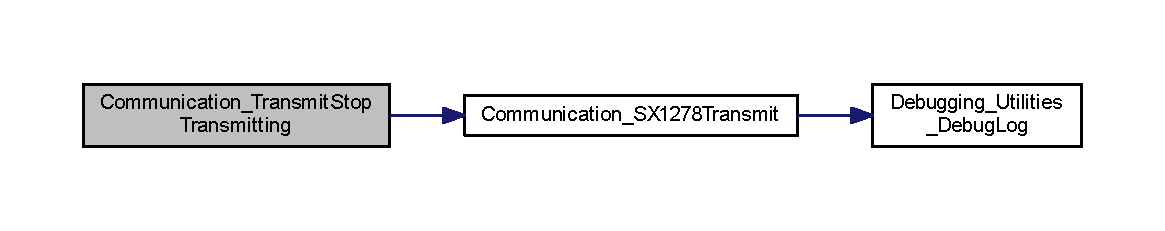
\includegraphics[width=350pt]{communication_8h_a7d368a63e53f4a1a63b166e6e97c7805_cgraph}
\end{center}
\end{figure}
Here is the caller graph for this function\+:\nopagebreak
\begin{figure}[H]
\begin{center}
\leavevmode
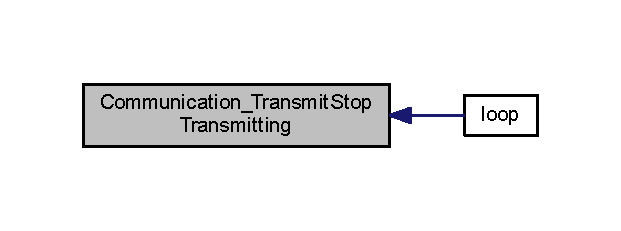
\includegraphics[width=298pt]{communication_8h_a7d368a63e53f4a1a63b166e6e97c7805_icgraph}
\end{center}
\end{figure}

\hypertarget{configuration_8cpp}{}\section{configuration.\+cpp File Reference}
\label{configuration_8cpp}\index{configuration.\+cpp@{configuration.\+cpp}}


This is the file in which all the static flags are stored. these are to be switched during prototype development.  


{\ttfamily \#include $<$Lo\+Ra\+Lib.\+h$>$}\newline
{\ttfamily \#include \char`\"{}configuration.\+h\char`\"{}}\newline
Include dependency graph for configuration.\+cpp\+:\nopagebreak
\begin{figure}[H]
\begin{center}
\leavevmode
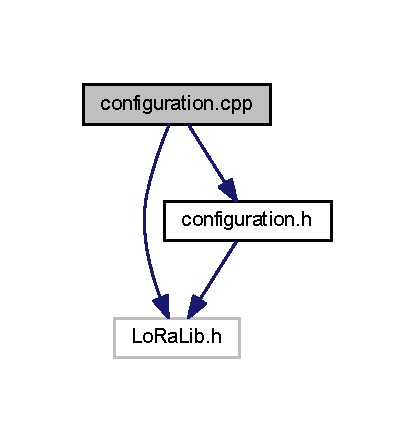
\includegraphics[width=199pt]{configuration_8cpp__incl}
\end{center}
\end{figure}
\subsection*{Variables}
\begin{DoxyCompactItemize}
\item 
bool \mbox{\hyperlink{configuration_8cpp_a117352cc494cc62c6b2f1882786a332c}{D\+E\+B\+UG}} = true
\begin{DoxyCompactList}\small\item\em Should the ground station output to serial. \end{DoxyCompactList}\item 
bool \mbox{\hyperlink{configuration_8cpp_ab1e5677d6b70e3965bdb8b1303d722f8}{A\+U\+T\+O\+M\+A\+T\+I\+C\+\_\+\+T\+U\+N\+I\+NG}} = true
\begin{DoxyCompactList}\small\item\em Should use the Transceiver settings message to tune its own antenna. \end{DoxyCompactList}\item 
S\+X1278 \mbox{\hyperlink{configuration_8cpp_a5f993a563f70b3c5508e11762006c2cf}{L\+O\+RA}} = new Lo\+Ra(7, 2, 3)
\item 
float \mbox{\hyperlink{configuration_8cpp_a6f812a7f3ce771172c19e67b93772474}{C\+A\+R\+R\+I\+E\+R\+\_\+\+F\+R\+E\+Q\+U\+E\+N\+CY}} = 434.\+0f
\begin{DoxyCompactList}\small\item\em Transmission frequency measured in M\+Hz (varies). \end{DoxyCompactList}\item 
float \mbox{\hyperlink{configuration_8cpp_a593e2609469ad2848c8eb2f99fedd6cd}{D\+E\+F\+A\+U\+L\+T\+\_\+\+C\+A\+R\+R\+I\+E\+R\+\_\+\+F\+R\+E\+Q\+U\+E\+N\+CY}} = 434.\+0f
\begin{DoxyCompactList}\small\item\em Transmission frequency measured in M\+Hz (constant). \end{DoxyCompactList}\item 
float \mbox{\hyperlink{configuration_8cpp_a8a1bb433d870a97dd5584108636cdbc3}{B\+A\+N\+D\+W\+I\+D\+TH}} = 62.\+5f
\begin{DoxyCompactList}\small\item\em Transmission bandwidth measured in K\+Hz. \end{DoxyCompactList}\item 
float \mbox{\hyperlink{configuration_8cpp_a8b4922dd8446574ca5548ec99a1f23e1}{C\+O\+N\+N\+E\+C\+T\+E\+D\+\_\+\+B\+A\+N\+D\+W\+I\+D\+TH}} = 7.\+8f
\begin{DoxyCompactList}\small\item\em Transmission bandwidth measured in K\+Hz (varies). \end{DoxyCompactList}\item 
int \mbox{\hyperlink{configuration_8cpp_a7171ec0721b810d80493f48ec7e73c00}{S\+P\+R\+E\+A\+D\+I\+N\+G\+\_\+\+F\+A\+C\+T\+OR}} = 12
\begin{DoxyCompactList}\small\item\em Chip duration. \end{DoxyCompactList}\item 
int \mbox{\hyperlink{configuration_8cpp_a058c5ebaef09467069080c27d0d07ff4}{C\+O\+D\+I\+N\+G\+\_\+\+R\+A\+TE}} = 8
\begin{DoxyCompactList}\small\item\em Cod erate. \end{DoxyCompactList}\item 
char \mbox{\hyperlink{configuration_8cpp_a8eb3cfcbe3656a266dc371537bcb4719}{S\+Y\+N\+C\+\_\+\+W\+O\+RD}} = 0x13
\begin{DoxyCompactList}\small\item\em Start of transmission frame preamble. \end{DoxyCompactList}\item 
int \mbox{\hyperlink{configuration_8cpp_adb47c06342602a39a68e0ea3e6786dc6}{O\+U\+T\+P\+U\+T\+\_\+\+P\+O\+W\+ER}} = 17
\begin{DoxyCompactList}\small\item\em Amount of power of radio frequency transmitted. \end{DoxyCompactList}\item 
String \mbox{\hyperlink{configuration_8cpp_a82c428085c407e360d82a73ad8847b63}{T\+R\+A\+N\+S\+M\+I\+S\+S\+I\+O\+N\+\_\+\+S\+I\+G\+N\+A\+T\+U\+RE}} = \char`\"{}F\+O\+S\+S\+A\+S\+AT-\/1\char`\"{}
\begin{DoxyCompactList}\small\item\em The unique identifyer for this satellite, used as a signature for transmissions. \end{DoxyCompactList}\end{DoxyCompactItemize}


\subsection{Detailed Description}
This is the file in which all the static flags are stored. these are to be switched during prototype development. 



\subsection{Variable Documentation}
\mbox{\Hypertarget{configuration_8cpp_ab1e5677d6b70e3965bdb8b1303d722f8}\label{configuration_8cpp_ab1e5677d6b70e3965bdb8b1303d722f8}} 
\index{configuration.\+cpp@{configuration.\+cpp}!A\+U\+T\+O\+M\+A\+T\+I\+C\+\_\+\+T\+U\+N\+I\+NG@{A\+U\+T\+O\+M\+A\+T\+I\+C\+\_\+\+T\+U\+N\+I\+NG}}
\index{A\+U\+T\+O\+M\+A\+T\+I\+C\+\_\+\+T\+U\+N\+I\+NG@{A\+U\+T\+O\+M\+A\+T\+I\+C\+\_\+\+T\+U\+N\+I\+NG}!configuration.\+cpp@{configuration.\+cpp}}
\subsubsection{\texorpdfstring{A\+U\+T\+O\+M\+A\+T\+I\+C\+\_\+\+T\+U\+N\+I\+NG}{AUTOMATIC\_TUNING}}
{\footnotesize\ttfamily bool A\+U\+T\+O\+M\+A\+T\+I\+C\+\_\+\+T\+U\+N\+I\+NG = true}



Should use the Transceiver settings message to tune its own antenna. 

This flag sets whether the ground station should tune itself from the Function Id \char`\"{}10\char`\"{} transmissions. only used for prototyping, if the tuning system fails to allow hardware debugging. \mbox{\Hypertarget{configuration_8cpp_a8a1bb433d870a97dd5584108636cdbc3}\label{configuration_8cpp_a8a1bb433d870a97dd5584108636cdbc3}} 
\index{configuration.\+cpp@{configuration.\+cpp}!B\+A\+N\+D\+W\+I\+D\+TH@{B\+A\+N\+D\+W\+I\+D\+TH}}
\index{B\+A\+N\+D\+W\+I\+D\+TH@{B\+A\+N\+D\+W\+I\+D\+TH}!configuration.\+cpp@{configuration.\+cpp}}
\subsubsection{\texorpdfstring{B\+A\+N\+D\+W\+I\+D\+TH}{BANDWIDTH}}
{\footnotesize\ttfamily float B\+A\+N\+D\+W\+I\+D\+TH = 62.\+5f}



Transmission bandwidth measured in K\+Hz. 

\mbox{\Hypertarget{configuration_8cpp_a6f812a7f3ce771172c19e67b93772474}\label{configuration_8cpp_a6f812a7f3ce771172c19e67b93772474}} 
\index{configuration.\+cpp@{configuration.\+cpp}!C\+A\+R\+R\+I\+E\+R\+\_\+\+F\+R\+E\+Q\+U\+E\+N\+CY@{C\+A\+R\+R\+I\+E\+R\+\_\+\+F\+R\+E\+Q\+U\+E\+N\+CY}}
\index{C\+A\+R\+R\+I\+E\+R\+\_\+\+F\+R\+E\+Q\+U\+E\+N\+CY@{C\+A\+R\+R\+I\+E\+R\+\_\+\+F\+R\+E\+Q\+U\+E\+N\+CY}!configuration.\+cpp@{configuration.\+cpp}}
\subsubsection{\texorpdfstring{C\+A\+R\+R\+I\+E\+R\+\_\+\+F\+R\+E\+Q\+U\+E\+N\+CY}{CARRIER\_FREQUENCY}}
{\footnotesize\ttfamily float C\+A\+R\+R\+I\+E\+R\+\_\+\+F\+R\+E\+Q\+U\+E\+N\+CY = 434.\+0f}



Transmission frequency measured in M\+Hz (varies). 

\mbox{\Hypertarget{configuration_8cpp_a058c5ebaef09467069080c27d0d07ff4}\label{configuration_8cpp_a058c5ebaef09467069080c27d0d07ff4}} 
\index{configuration.\+cpp@{configuration.\+cpp}!C\+O\+D\+I\+N\+G\+\_\+\+R\+A\+TE@{C\+O\+D\+I\+N\+G\+\_\+\+R\+A\+TE}}
\index{C\+O\+D\+I\+N\+G\+\_\+\+R\+A\+TE@{C\+O\+D\+I\+N\+G\+\_\+\+R\+A\+TE}!configuration.\+cpp@{configuration.\+cpp}}
\subsubsection{\texorpdfstring{C\+O\+D\+I\+N\+G\+\_\+\+R\+A\+TE}{CODING\_RATE}}
{\footnotesize\ttfamily int C\+O\+D\+I\+N\+G\+\_\+\+R\+A\+TE = 8}



Cod erate. 

\mbox{\Hypertarget{configuration_8cpp_a8b4922dd8446574ca5548ec99a1f23e1}\label{configuration_8cpp_a8b4922dd8446574ca5548ec99a1f23e1}} 
\index{configuration.\+cpp@{configuration.\+cpp}!C\+O\+N\+N\+E\+C\+T\+E\+D\+\_\+\+B\+A\+N\+D\+W\+I\+D\+TH@{C\+O\+N\+N\+E\+C\+T\+E\+D\+\_\+\+B\+A\+N\+D\+W\+I\+D\+TH}}
\index{C\+O\+N\+N\+E\+C\+T\+E\+D\+\_\+\+B\+A\+N\+D\+W\+I\+D\+TH@{C\+O\+N\+N\+E\+C\+T\+E\+D\+\_\+\+B\+A\+N\+D\+W\+I\+D\+TH}!configuration.\+cpp@{configuration.\+cpp}}
\subsubsection{\texorpdfstring{C\+O\+N\+N\+E\+C\+T\+E\+D\+\_\+\+B\+A\+N\+D\+W\+I\+D\+TH}{CONNECTED\_BANDWIDTH}}
{\footnotesize\ttfamily float C\+O\+N\+N\+E\+C\+T\+E\+D\+\_\+\+B\+A\+N\+D\+W\+I\+D\+TH = 7.\+8f}



Transmission bandwidth measured in K\+Hz (varies). 

\mbox{\Hypertarget{configuration_8cpp_a117352cc494cc62c6b2f1882786a332c}\label{configuration_8cpp_a117352cc494cc62c6b2f1882786a332c}} 
\index{configuration.\+cpp@{configuration.\+cpp}!D\+E\+B\+UG@{D\+E\+B\+UG}}
\index{D\+E\+B\+UG@{D\+E\+B\+UG}!configuration.\+cpp@{configuration.\+cpp}}
\subsubsection{\texorpdfstring{D\+E\+B\+UG}{DEBUG}}
{\footnotesize\ttfamily bool D\+E\+B\+UG = true}



Should the ground station output to serial. 

This flag sets whether the ground station should print through the Debug\+Log via serial. Upon prototype finishing, this should be removed along with the debugging functions, this servers as a temporary development flag. \mbox{\Hypertarget{configuration_8cpp_a593e2609469ad2848c8eb2f99fedd6cd}\label{configuration_8cpp_a593e2609469ad2848c8eb2f99fedd6cd}} 
\index{configuration.\+cpp@{configuration.\+cpp}!D\+E\+F\+A\+U\+L\+T\+\_\+\+C\+A\+R\+R\+I\+E\+R\+\_\+\+F\+R\+E\+Q\+U\+E\+N\+CY@{D\+E\+F\+A\+U\+L\+T\+\_\+\+C\+A\+R\+R\+I\+E\+R\+\_\+\+F\+R\+E\+Q\+U\+E\+N\+CY}}
\index{D\+E\+F\+A\+U\+L\+T\+\_\+\+C\+A\+R\+R\+I\+E\+R\+\_\+\+F\+R\+E\+Q\+U\+E\+N\+CY@{D\+E\+F\+A\+U\+L\+T\+\_\+\+C\+A\+R\+R\+I\+E\+R\+\_\+\+F\+R\+E\+Q\+U\+E\+N\+CY}!configuration.\+cpp@{configuration.\+cpp}}
\subsubsection{\texorpdfstring{D\+E\+F\+A\+U\+L\+T\+\_\+\+C\+A\+R\+R\+I\+E\+R\+\_\+\+F\+R\+E\+Q\+U\+E\+N\+CY}{DEFAULT\_CARRIER\_FREQUENCY}}
{\footnotesize\ttfamily float D\+E\+F\+A\+U\+L\+T\+\_\+\+C\+A\+R\+R\+I\+E\+R\+\_\+\+F\+R\+E\+Q\+U\+E\+N\+CY = 434.\+0f}



Transmission frequency measured in M\+Hz (constant). 

\mbox{\Hypertarget{configuration_8cpp_a5f993a563f70b3c5508e11762006c2cf}\label{configuration_8cpp_a5f993a563f70b3c5508e11762006c2cf}} 
\index{configuration.\+cpp@{configuration.\+cpp}!L\+O\+RA@{L\+O\+RA}}
\index{L\+O\+RA@{L\+O\+RA}!configuration.\+cpp@{configuration.\+cpp}}
\subsubsection{\texorpdfstring{L\+O\+RA}{LORA}}
{\footnotesize\ttfamily S\+X1278 L\+O\+RA = new Lo\+Ra(7, 2, 3)}

S\+X1278 pin layout  N\+SS P\+IN = 7 D\+I\+O0 P\+IN = 2 D\+I\+O1 P\+IN = 3 \mbox{\Hypertarget{configuration_8cpp_adb47c06342602a39a68e0ea3e6786dc6}\label{configuration_8cpp_adb47c06342602a39a68e0ea3e6786dc6}} 
\index{configuration.\+cpp@{configuration.\+cpp}!O\+U\+T\+P\+U\+T\+\_\+\+P\+O\+W\+ER@{O\+U\+T\+P\+U\+T\+\_\+\+P\+O\+W\+ER}}
\index{O\+U\+T\+P\+U\+T\+\_\+\+P\+O\+W\+ER@{O\+U\+T\+P\+U\+T\+\_\+\+P\+O\+W\+ER}!configuration.\+cpp@{configuration.\+cpp}}
\subsubsection{\texorpdfstring{O\+U\+T\+P\+U\+T\+\_\+\+P\+O\+W\+ER}{OUTPUT\_POWER}}
{\footnotesize\ttfamily int O\+U\+T\+P\+U\+T\+\_\+\+P\+O\+W\+ER = 17}



Amount of power of radio frequency transmitted. 

\mbox{\Hypertarget{configuration_8cpp_a7171ec0721b810d80493f48ec7e73c00}\label{configuration_8cpp_a7171ec0721b810d80493f48ec7e73c00}} 
\index{configuration.\+cpp@{configuration.\+cpp}!S\+P\+R\+E\+A\+D\+I\+N\+G\+\_\+\+F\+A\+C\+T\+OR@{S\+P\+R\+E\+A\+D\+I\+N\+G\+\_\+\+F\+A\+C\+T\+OR}}
\index{S\+P\+R\+E\+A\+D\+I\+N\+G\+\_\+\+F\+A\+C\+T\+OR@{S\+P\+R\+E\+A\+D\+I\+N\+G\+\_\+\+F\+A\+C\+T\+OR}!configuration.\+cpp@{configuration.\+cpp}}
\subsubsection{\texorpdfstring{S\+P\+R\+E\+A\+D\+I\+N\+G\+\_\+\+F\+A\+C\+T\+OR}{SPREADING\_FACTOR}}
{\footnotesize\ttfamily int S\+P\+R\+E\+A\+D\+I\+N\+G\+\_\+\+F\+A\+C\+T\+OR = 12}



Chip duration. 

\mbox{\Hypertarget{configuration_8cpp_a8eb3cfcbe3656a266dc371537bcb4719}\label{configuration_8cpp_a8eb3cfcbe3656a266dc371537bcb4719}} 
\index{configuration.\+cpp@{configuration.\+cpp}!S\+Y\+N\+C\+\_\+\+W\+O\+RD@{S\+Y\+N\+C\+\_\+\+W\+O\+RD}}
\index{S\+Y\+N\+C\+\_\+\+W\+O\+RD@{S\+Y\+N\+C\+\_\+\+W\+O\+RD}!configuration.\+cpp@{configuration.\+cpp}}
\subsubsection{\texorpdfstring{S\+Y\+N\+C\+\_\+\+W\+O\+RD}{SYNC\_WORD}}
{\footnotesize\ttfamily char S\+Y\+N\+C\+\_\+\+W\+O\+RD = 0x13}



Start of transmission frame preamble. 

\mbox{\Hypertarget{configuration_8cpp_a82c428085c407e360d82a73ad8847b63}\label{configuration_8cpp_a82c428085c407e360d82a73ad8847b63}} 
\index{configuration.\+cpp@{configuration.\+cpp}!T\+R\+A\+N\+S\+M\+I\+S\+S\+I\+O\+N\+\_\+\+S\+I\+G\+N\+A\+T\+U\+RE@{T\+R\+A\+N\+S\+M\+I\+S\+S\+I\+O\+N\+\_\+\+S\+I\+G\+N\+A\+T\+U\+RE}}
\index{T\+R\+A\+N\+S\+M\+I\+S\+S\+I\+O\+N\+\_\+\+S\+I\+G\+N\+A\+T\+U\+RE@{T\+R\+A\+N\+S\+M\+I\+S\+S\+I\+O\+N\+\_\+\+S\+I\+G\+N\+A\+T\+U\+RE}!configuration.\+cpp@{configuration.\+cpp}}
\subsubsection{\texorpdfstring{T\+R\+A\+N\+S\+M\+I\+S\+S\+I\+O\+N\+\_\+\+S\+I\+G\+N\+A\+T\+U\+RE}{TRANSMISSION\_SIGNATURE}}
{\footnotesize\ttfamily String T\+R\+A\+N\+S\+M\+I\+S\+S\+I\+O\+N\+\_\+\+S\+I\+G\+N\+A\+T\+U\+RE = \char`\"{}F\+O\+S\+S\+A\+S\+AT-\/1\char`\"{}}



The unique identifyer for this satellite, used as a signature for transmissions. 


\hypertarget{configuration_8h}{}\section{configuration.\+h File Reference}
\label{configuration_8h}\index{configuration.\+h@{configuration.\+h}}
{\ttfamily \#include $<$Lo\+Ra\+Lib.\+h$>$}\newline
Include dependency graph for configuration.\+h\+:\nopagebreak
\begin{figure}[H]
\begin{center}
\leavevmode
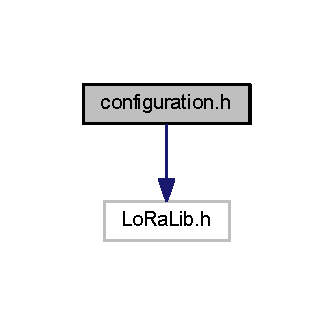
\includegraphics[width=160pt]{configuration_8h__incl}
\end{center}
\end{figure}
This graph shows which files directly or indirectly include this file\+:\nopagebreak
\begin{figure}[H]
\begin{center}
\leavevmode
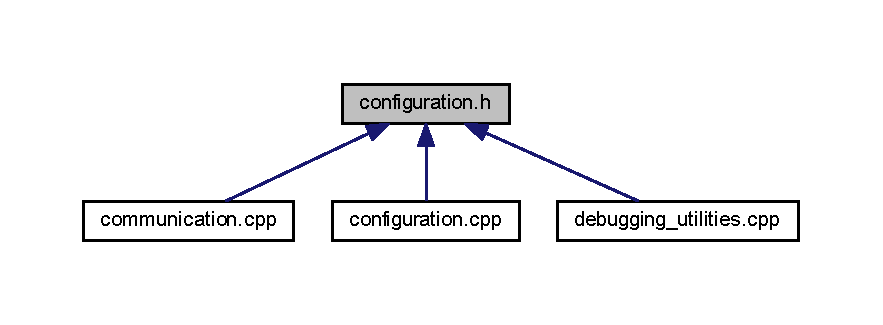
\includegraphics[width=350pt]{configuration_8h__dep__incl}
\end{center}
\end{figure}
\subsection*{Variables}
\begin{DoxyCompactItemize}
\item 
bool \mbox{\hyperlink{configuration_8h_a117352cc494cc62c6b2f1882786a332c}{D\+E\+B\+UG}}
\begin{DoxyCompactList}\small\item\em Should the ground station output to serial. \end{DoxyCompactList}\item 
bool \mbox{\hyperlink{configuration_8h_ab1e5677d6b70e3965bdb8b1303d722f8}{A\+U\+T\+O\+M\+A\+T\+I\+C\+\_\+\+T\+U\+N\+I\+NG}}
\begin{DoxyCompactList}\small\item\em Should use the Transceiver settings message to tune its own antenna. \end{DoxyCompactList}\item 
S\+X1278 \mbox{\hyperlink{configuration_8h_a5f993a563f70b3c5508e11762006c2cf}{L\+O\+RA}}
\item 
float \mbox{\hyperlink{configuration_8h_a6f812a7f3ce771172c19e67b93772474}{C\+A\+R\+R\+I\+E\+R\+\_\+\+F\+R\+E\+Q\+U\+E\+N\+CY}}
\begin{DoxyCompactList}\small\item\em Transmission frequency measured in M\+Hz (varies). \end{DoxyCompactList}\item 
float \mbox{\hyperlink{configuration_8h_a426167635a8daaf1b926747538e1379a}{L\+O\+C\+A\+T\+I\+O\+N\+\_\+\+B\+A\+N\+D\+W\+I\+D\+TH}}
\item 
float \mbox{\hyperlink{configuration_8h_a8a1bb433d870a97dd5584108636cdbc3}{B\+A\+N\+D\+W\+I\+D\+TH}}
\begin{DoxyCompactList}\small\item\em Transmission bandwidth measured in K\+Hz. \end{DoxyCompactList}\item 
int \mbox{\hyperlink{configuration_8h_a7171ec0721b810d80493f48ec7e73c00}{S\+P\+R\+E\+A\+D\+I\+N\+G\+\_\+\+F\+A\+C\+T\+OR}}
\begin{DoxyCompactList}\small\item\em Chip duration. \end{DoxyCompactList}\item 
int \mbox{\hyperlink{configuration_8h_a058c5ebaef09467069080c27d0d07ff4}{C\+O\+D\+I\+N\+G\+\_\+\+R\+A\+TE}}
\begin{DoxyCompactList}\small\item\em Cod erate. \end{DoxyCompactList}\item 
char \mbox{\hyperlink{configuration_8h_a8eb3cfcbe3656a266dc371537bcb4719}{S\+Y\+N\+C\+\_\+\+W\+O\+RD}}
\begin{DoxyCompactList}\small\item\em Start of transmission frame preamble. \end{DoxyCompactList}\item 
int \mbox{\hyperlink{configuration_8h_adb47c06342602a39a68e0ea3e6786dc6}{O\+U\+T\+P\+U\+T\+\_\+\+P\+O\+W\+ER}}
\begin{DoxyCompactList}\small\item\em Amount of power of radio frequency transmitted. \end{DoxyCompactList}\item 
String \mbox{\hyperlink{configuration_8h_a82c428085c407e360d82a73ad8847b63}{T\+R\+A\+N\+S\+M\+I\+S\+S\+I\+O\+N\+\_\+\+S\+I\+G\+N\+A\+T\+U\+RE}}
\begin{DoxyCompactList}\small\item\em The unique identifyer for this satellite, used as a signature for transmissions. \end{DoxyCompactList}\end{DoxyCompactItemize}


\subsection{Variable Documentation}
\mbox{\Hypertarget{configuration_8h_ab1e5677d6b70e3965bdb8b1303d722f8}\label{configuration_8h_ab1e5677d6b70e3965bdb8b1303d722f8}} 
\index{configuration.\+h@{configuration.\+h}!A\+U\+T\+O\+M\+A\+T\+I\+C\+\_\+\+T\+U\+N\+I\+NG@{A\+U\+T\+O\+M\+A\+T\+I\+C\+\_\+\+T\+U\+N\+I\+NG}}
\index{A\+U\+T\+O\+M\+A\+T\+I\+C\+\_\+\+T\+U\+N\+I\+NG@{A\+U\+T\+O\+M\+A\+T\+I\+C\+\_\+\+T\+U\+N\+I\+NG}!configuration.\+h@{configuration.\+h}}
\subsubsection{\texorpdfstring{A\+U\+T\+O\+M\+A\+T\+I\+C\+\_\+\+T\+U\+N\+I\+NG}{AUTOMATIC\_TUNING}}
{\footnotesize\ttfamily bool A\+U\+T\+O\+M\+A\+T\+I\+C\+\_\+\+T\+U\+N\+I\+NG}



Should use the Transceiver settings message to tune its own antenna. 

This flag sets whether the ground station should tune itself from the Function Id \char`\"{}10\char`\"{} transmissions. only used for prototyping, if the tuning system fails to allow hardware debugging. \mbox{\Hypertarget{configuration_8h_a8a1bb433d870a97dd5584108636cdbc3}\label{configuration_8h_a8a1bb433d870a97dd5584108636cdbc3}} 
\index{configuration.\+h@{configuration.\+h}!B\+A\+N\+D\+W\+I\+D\+TH@{B\+A\+N\+D\+W\+I\+D\+TH}}
\index{B\+A\+N\+D\+W\+I\+D\+TH@{B\+A\+N\+D\+W\+I\+D\+TH}!configuration.\+h@{configuration.\+h}}
\subsubsection{\texorpdfstring{B\+A\+N\+D\+W\+I\+D\+TH}{BANDWIDTH}}
{\footnotesize\ttfamily float B\+A\+N\+D\+W\+I\+D\+TH}



Transmission bandwidth measured in K\+Hz. 

\mbox{\Hypertarget{configuration_8h_a6f812a7f3ce771172c19e67b93772474}\label{configuration_8h_a6f812a7f3ce771172c19e67b93772474}} 
\index{configuration.\+h@{configuration.\+h}!C\+A\+R\+R\+I\+E\+R\+\_\+\+F\+R\+E\+Q\+U\+E\+N\+CY@{C\+A\+R\+R\+I\+E\+R\+\_\+\+F\+R\+E\+Q\+U\+E\+N\+CY}}
\index{C\+A\+R\+R\+I\+E\+R\+\_\+\+F\+R\+E\+Q\+U\+E\+N\+CY@{C\+A\+R\+R\+I\+E\+R\+\_\+\+F\+R\+E\+Q\+U\+E\+N\+CY}!configuration.\+h@{configuration.\+h}}
\subsubsection{\texorpdfstring{C\+A\+R\+R\+I\+E\+R\+\_\+\+F\+R\+E\+Q\+U\+E\+N\+CY}{CARRIER\_FREQUENCY}}
{\footnotesize\ttfamily float C\+A\+R\+R\+I\+E\+R\+\_\+\+F\+R\+E\+Q\+U\+E\+N\+CY}



Transmission frequency measured in M\+Hz (varies). 

\mbox{\Hypertarget{configuration_8h_a058c5ebaef09467069080c27d0d07ff4}\label{configuration_8h_a058c5ebaef09467069080c27d0d07ff4}} 
\index{configuration.\+h@{configuration.\+h}!C\+O\+D\+I\+N\+G\+\_\+\+R\+A\+TE@{C\+O\+D\+I\+N\+G\+\_\+\+R\+A\+TE}}
\index{C\+O\+D\+I\+N\+G\+\_\+\+R\+A\+TE@{C\+O\+D\+I\+N\+G\+\_\+\+R\+A\+TE}!configuration.\+h@{configuration.\+h}}
\subsubsection{\texorpdfstring{C\+O\+D\+I\+N\+G\+\_\+\+R\+A\+TE}{CODING\_RATE}}
{\footnotesize\ttfamily int C\+O\+D\+I\+N\+G\+\_\+\+R\+A\+TE}



Cod erate. 

\mbox{\Hypertarget{configuration_8h_a117352cc494cc62c6b2f1882786a332c}\label{configuration_8h_a117352cc494cc62c6b2f1882786a332c}} 
\index{configuration.\+h@{configuration.\+h}!D\+E\+B\+UG@{D\+E\+B\+UG}}
\index{D\+E\+B\+UG@{D\+E\+B\+UG}!configuration.\+h@{configuration.\+h}}
\subsubsection{\texorpdfstring{D\+E\+B\+UG}{DEBUG}}
{\footnotesize\ttfamily bool D\+E\+B\+UG}



Should the ground station output to serial. 

This flag sets whether the ground station should print through the Debug\+Log via serial. Upon prototype finishing, this should be removed along with the debugging functions, this servers as a temporary development flag. \mbox{\Hypertarget{configuration_8h_a426167635a8daaf1b926747538e1379a}\label{configuration_8h_a426167635a8daaf1b926747538e1379a}} 
\index{configuration.\+h@{configuration.\+h}!L\+O\+C\+A\+T\+I\+O\+N\+\_\+\+B\+A\+N\+D\+W\+I\+D\+TH@{L\+O\+C\+A\+T\+I\+O\+N\+\_\+\+B\+A\+N\+D\+W\+I\+D\+TH}}
\index{L\+O\+C\+A\+T\+I\+O\+N\+\_\+\+B\+A\+N\+D\+W\+I\+D\+TH@{L\+O\+C\+A\+T\+I\+O\+N\+\_\+\+B\+A\+N\+D\+W\+I\+D\+TH}!configuration.\+h@{configuration.\+h}}
\subsubsection{\texorpdfstring{L\+O\+C\+A\+T\+I\+O\+N\+\_\+\+B\+A\+N\+D\+W\+I\+D\+TH}{LOCATION\_BANDWIDTH}}
{\footnotesize\ttfamily float L\+O\+C\+A\+T\+I\+O\+N\+\_\+\+B\+A\+N\+D\+W\+I\+D\+TH}

\mbox{\Hypertarget{configuration_8h_a5f993a563f70b3c5508e11762006c2cf}\label{configuration_8h_a5f993a563f70b3c5508e11762006c2cf}} 
\index{configuration.\+h@{configuration.\+h}!L\+O\+RA@{L\+O\+RA}}
\index{L\+O\+RA@{L\+O\+RA}!configuration.\+h@{configuration.\+h}}
\subsubsection{\texorpdfstring{L\+O\+RA}{LORA}}
{\footnotesize\ttfamily S\+X1278 L\+O\+RA}

S\+X1278 pin layout  N\+SS P\+IN = 7 D\+I\+O0 P\+IN = 2 D\+I\+O1 P\+IN = 3 \mbox{\Hypertarget{configuration_8h_adb47c06342602a39a68e0ea3e6786dc6}\label{configuration_8h_adb47c06342602a39a68e0ea3e6786dc6}} 
\index{configuration.\+h@{configuration.\+h}!O\+U\+T\+P\+U\+T\+\_\+\+P\+O\+W\+ER@{O\+U\+T\+P\+U\+T\+\_\+\+P\+O\+W\+ER}}
\index{O\+U\+T\+P\+U\+T\+\_\+\+P\+O\+W\+ER@{O\+U\+T\+P\+U\+T\+\_\+\+P\+O\+W\+ER}!configuration.\+h@{configuration.\+h}}
\subsubsection{\texorpdfstring{O\+U\+T\+P\+U\+T\+\_\+\+P\+O\+W\+ER}{OUTPUT\_POWER}}
{\footnotesize\ttfamily int O\+U\+T\+P\+U\+T\+\_\+\+P\+O\+W\+ER}



Amount of power of radio frequency transmitted. 

\mbox{\Hypertarget{configuration_8h_a7171ec0721b810d80493f48ec7e73c00}\label{configuration_8h_a7171ec0721b810d80493f48ec7e73c00}} 
\index{configuration.\+h@{configuration.\+h}!S\+P\+R\+E\+A\+D\+I\+N\+G\+\_\+\+F\+A\+C\+T\+OR@{S\+P\+R\+E\+A\+D\+I\+N\+G\+\_\+\+F\+A\+C\+T\+OR}}
\index{S\+P\+R\+E\+A\+D\+I\+N\+G\+\_\+\+F\+A\+C\+T\+OR@{S\+P\+R\+E\+A\+D\+I\+N\+G\+\_\+\+F\+A\+C\+T\+OR}!configuration.\+h@{configuration.\+h}}
\subsubsection{\texorpdfstring{S\+P\+R\+E\+A\+D\+I\+N\+G\+\_\+\+F\+A\+C\+T\+OR}{SPREADING\_FACTOR}}
{\footnotesize\ttfamily int S\+P\+R\+E\+A\+D\+I\+N\+G\+\_\+\+F\+A\+C\+T\+OR}



Chip duration. 

\mbox{\Hypertarget{configuration_8h_a8eb3cfcbe3656a266dc371537bcb4719}\label{configuration_8h_a8eb3cfcbe3656a266dc371537bcb4719}} 
\index{configuration.\+h@{configuration.\+h}!S\+Y\+N\+C\+\_\+\+W\+O\+RD@{S\+Y\+N\+C\+\_\+\+W\+O\+RD}}
\index{S\+Y\+N\+C\+\_\+\+W\+O\+RD@{S\+Y\+N\+C\+\_\+\+W\+O\+RD}!configuration.\+h@{configuration.\+h}}
\subsubsection{\texorpdfstring{S\+Y\+N\+C\+\_\+\+W\+O\+RD}{SYNC\_WORD}}
{\footnotesize\ttfamily char S\+Y\+N\+C\+\_\+\+W\+O\+RD}



Start of transmission frame preamble. 

\mbox{\Hypertarget{configuration_8h_a82c428085c407e360d82a73ad8847b63}\label{configuration_8h_a82c428085c407e360d82a73ad8847b63}} 
\index{configuration.\+h@{configuration.\+h}!T\+R\+A\+N\+S\+M\+I\+S\+S\+I\+O\+N\+\_\+\+S\+I\+G\+N\+A\+T\+U\+RE@{T\+R\+A\+N\+S\+M\+I\+S\+S\+I\+O\+N\+\_\+\+S\+I\+G\+N\+A\+T\+U\+RE}}
\index{T\+R\+A\+N\+S\+M\+I\+S\+S\+I\+O\+N\+\_\+\+S\+I\+G\+N\+A\+T\+U\+RE@{T\+R\+A\+N\+S\+M\+I\+S\+S\+I\+O\+N\+\_\+\+S\+I\+G\+N\+A\+T\+U\+RE}!configuration.\+h@{configuration.\+h}}
\subsubsection{\texorpdfstring{T\+R\+A\+N\+S\+M\+I\+S\+S\+I\+O\+N\+\_\+\+S\+I\+G\+N\+A\+T\+U\+RE}{TRANSMISSION\_SIGNATURE}}
{\footnotesize\ttfamily String T\+R\+A\+N\+S\+M\+I\+S\+S\+I\+O\+N\+\_\+\+S\+I\+G\+N\+A\+T\+U\+RE}



The unique identifyer for this satellite, used as a signature for transmissions. 


\hypertarget{debugging__utilities_8cpp}{}\section{debugging\+\_\+utilities.\+cpp File Reference}
\label{debugging__utilities_8cpp}\index{debugging\+\_\+utilities.\+cpp@{debugging\+\_\+utilities.\+cpp}}


Serial println abstraction with D\+E\+B\+UG configuration switch. This is so all printlns can be traced.  


{\ttfamily \#include $<$Arduino.\+h$>$}\newline
{\ttfamily \#include $<$Lo\+Ra\+Lib.\+h$>$}\newline
{\ttfamily \#include \char`\"{}configuration.\+h\char`\"{}}\newline
{\ttfamily \#include \char`\"{}debugging\+\_\+utilities.\+h\char`\"{}}\newline
Include dependency graph for debugging\+\_\+utilities.\+cpp\+:\nopagebreak
\begin{figure}[H]
\begin{center}
\leavevmode
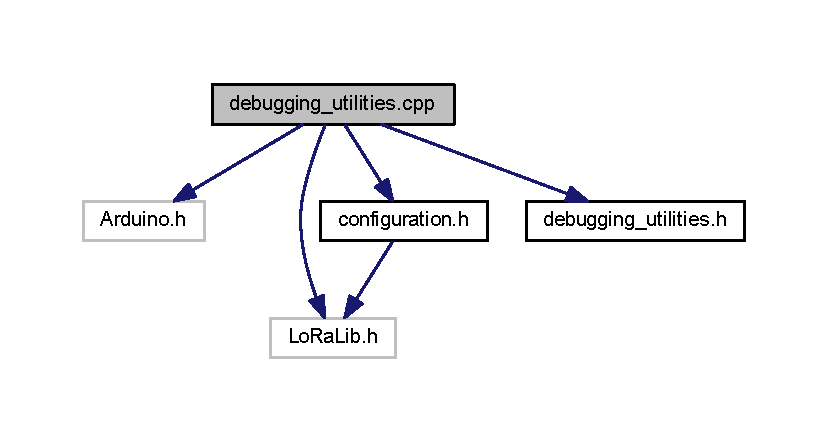
\includegraphics[width=350pt]{debugging__utilities_8cpp__incl}
\end{center}
\end{figure}
\subsection*{Functions}
\begin{DoxyCompactItemize}
\item 
void \mbox{\hyperlink{debugging__utilities_8cpp_ac9c910db5861d4a642082aa29dfae40a}{Debugging\+\_\+\+Utilities\+\_\+\+Debug\+Log}} (String in\+Line)
\end{DoxyCompactItemize}


\subsection{Detailed Description}
Serial println abstraction with D\+E\+B\+UG configuration switch. This is so all printlns can be traced. 



\subsection{Function Documentation}
\mbox{\Hypertarget{debugging__utilities_8cpp_ac9c910db5861d4a642082aa29dfae40a}\label{debugging__utilities_8cpp_ac9c910db5861d4a642082aa29dfae40a}} 
\index{debugging\+\_\+utilities.\+cpp@{debugging\+\_\+utilities.\+cpp}!Debugging\+\_\+\+Utilities\+\_\+\+Debug\+Log@{Debugging\+\_\+\+Utilities\+\_\+\+Debug\+Log}}
\index{Debugging\+\_\+\+Utilities\+\_\+\+Debug\+Log@{Debugging\+\_\+\+Utilities\+\_\+\+Debug\+Log}!debugging\+\_\+utilities.\+cpp@{debugging\+\_\+utilities.\+cpp}}
\subsubsection{\texorpdfstring{Debugging\+\_\+\+Utilities\+\_\+\+Debug\+Log()}{Debugging\_Utilities\_DebugLog()}}
{\footnotesize\ttfamily void Debugging\+\_\+\+Utilities\+\_\+\+Debug\+Log (\begin{DoxyParamCaption}\item[{String}]{in\+Line }\end{DoxyParamCaption})}

Here is the caller graph for this function\+:\nopagebreak
\begin{figure}[H]
\begin{center}
\leavevmode
\includegraphics[width=350pt]{debugging__utilities_8cpp_ac9c910db5861d4a642082aa29dfae40a_icgraph}
\end{center}
\end{figure}

\hypertarget{debugging__utilities_8h}{}\section{debugging\+\_\+utilities.\+h File Reference}
\label{debugging__utilities_8h}\index{debugging\+\_\+utilities.\+h@{debugging\+\_\+utilities.\+h}}
This graph shows which files directly or indirectly include this file\+:\nopagebreak
\begin{figure}[H]
\begin{center}
\leavevmode
\includegraphics[width=350pt]{debugging__utilities_8h__dep__incl}
\end{center}
\end{figure}
\subsection*{Functions}
\begin{DoxyCompactItemize}
\item 
void \mbox{\hyperlink{debugging__utilities_8h_ac9c910db5861d4a642082aa29dfae40a}{Debugging\+\_\+\+Utilities\+\_\+\+Debug\+Log}} (String in\+Line)
\end{DoxyCompactItemize}


\subsection{Function Documentation}
\mbox{\Hypertarget{debugging__utilities_8h_ac9c910db5861d4a642082aa29dfae40a}\label{debugging__utilities_8h_ac9c910db5861d4a642082aa29dfae40a}} 
\index{debugging\+\_\+utilities.\+h@{debugging\+\_\+utilities.\+h}!Debugging\+\_\+\+Utilities\+\_\+\+Debug\+Log@{Debugging\+\_\+\+Utilities\+\_\+\+Debug\+Log}}
\index{Debugging\+\_\+\+Utilities\+\_\+\+Debug\+Log@{Debugging\+\_\+\+Utilities\+\_\+\+Debug\+Log}!debugging\+\_\+utilities.\+h@{debugging\+\_\+utilities.\+h}}
\subsubsection{\texorpdfstring{Debugging\+\_\+\+Utilities\+\_\+\+Debug\+Log()}{Debugging\_Utilities\_DebugLog()}}
{\footnotesize\ttfamily void Debugging\+\_\+\+Utilities\+\_\+\+Debug\+Log (\begin{DoxyParamCaption}\item[{String}]{in\+Line }\end{DoxyParamCaption})}

Here is the caller graph for this function\+:\nopagebreak
\begin{figure}[H]
\begin{center}
\leavevmode
\includegraphics[width=350pt]{debugging__utilities_8h_ac9c910db5861d4a642082aa29dfae40a_icgraph}
\end{center}
\end{figure}

\hypertarget{ground__station_8cpp}{}\section{ground\+\_\+station.\+cpp File Reference}
\label{ground__station_8cpp}\index{ground\+\_\+station.\+cpp@{ground\+\_\+station.\+cpp}}


This is the main code starting point. It manages the state of the ground station.  


{\ttfamily \#include $<$Lo\+Ra\+Lib.\+h$>$}\newline
{\ttfamily \#include \char`\"{}configuration.\+h\char`\"{}}\newline
{\ttfamily \#include \char`\"{}debugging\+\_\+utilities.\+h\char`\"{}}\newline
{\ttfamily \#include \char`\"{}state\+\_\+machine\+\_\+declerations.\+h\char`\"{}}\newline
{\ttfamily \#include \char`\"{}communication.\+h\char`\"{}}\newline
Include dependency graph for ground\+\_\+station.\+cpp\+:\nopagebreak
\begin{figure}[H]
\begin{center}
\leavevmode
\includegraphics[width=350pt]{ground__station_8cpp__incl}
\end{center}
\end{figure}
\subsection*{Functions}
\begin{DoxyCompactItemize}
\item 
void \mbox{\hyperlink{ground__station_8cpp_a4fc01d736fe50cf5b977f755b675f11d}{setup}} ()
\item 
void \mbox{\hyperlink{ground__station_8cpp_afe461d27b9c48d5921c00d521181f12f}{loop}} ()
\end{DoxyCompactItemize}


\subsection{Detailed Description}
This is the main code starting point. It manages the state of the ground station. 



\subsection{Function Documentation}
\mbox{\Hypertarget{ground__station_8cpp_afe461d27b9c48d5921c00d521181f12f}\label{ground__station_8cpp_afe461d27b9c48d5921c00d521181f12f}} 
\index{ground\+\_\+station.\+cpp@{ground\+\_\+station.\+cpp}!loop@{loop}}
\index{loop@{loop}!ground\+\_\+station.\+cpp@{ground\+\_\+station.\+cpp}}
\subsubsection{\texorpdfstring{loop()}{loop()}}
{\footnotesize\ttfamily void loop (\begin{DoxyParamCaption}{ }\end{DoxyParamCaption})}

The looping function.
\begin{DoxyItemize}
\item Where the L\+O\+RA transceiver\textquotesingle{}s state is managed. Where the L\+O\+RA transceiver is tuned on the function id \char`\"{}10\char`\"{} transmission. If the communication is lost to the satellite, this manages the switching between low and high bandwidth modes.
\end{DoxyItemize}

\begin{DoxyRefDesc}{Test}
\item[\mbox{\hyperlink{test__test000003}{Test}}]See how it behaves without a S\+X1278 interface. 

Test each function ID and ensure it prints to debug the correct functions. 

Ensure that the frequency error we receive on a packet is suitable for tuning with. 

Does changing the frequency of the L\+O\+RA class at runtime work? 

D\+Oes changing the bandwidth of the L\+O\+RA class at runtime work? \end{DoxyRefDesc}
Here is the call graph for this function\+:\nopagebreak
\begin{figure}[H]
\begin{center}
\leavevmode
\includegraphics[width=350pt]{ground__station_8cpp_afe461d27b9c48d5921c00d521181f12f_cgraph}
\end{center}
\end{figure}
\mbox{\Hypertarget{ground__station_8cpp_a4fc01d736fe50cf5b977f755b675f11d}\label{ground__station_8cpp_a4fc01d736fe50cf5b977f755b675f11d}} 
\index{ground\+\_\+station.\+cpp@{ground\+\_\+station.\+cpp}!setup@{setup}}
\index{setup@{setup}!ground\+\_\+station.\+cpp@{ground\+\_\+station.\+cpp}}
\subsubsection{\texorpdfstring{setup()}{setup()}}
{\footnotesize\ttfamily void setup (\begin{DoxyParamCaption}{ }\end{DoxyParamCaption})}

The starting point of the entire code base.

Called upon arduino startup.
\begin{DoxyItemize}
\item Configures the S\+X1278 chip pin layout and settings.
\end{DoxyItemize}

\begin{DoxyRefDesc}{Test}
\item[\mbox{\hyperlink{test__test000002}{Test}}]Test ground station with no S\+X1278 chip connected to see how it fails. \end{DoxyRefDesc}
Here is the call graph for this function\+:\nopagebreak
\begin{figure}[H]
\begin{center}
\leavevmode
\includegraphics[width=257pt]{ground__station_8cpp_a4fc01d736fe50cf5b977f755b675f11d_cgraph}
\end{center}
\end{figure}

\hypertarget{mainpage_8dox}{}\section{mainpage.\+dox File Reference}
\label{mainpage_8dox}\index{mainpage.\+dox@{mainpage.\+dox}}

\hypertarget{state__machine__declerations_8cpp}{}\section{state\+\_\+machine\+\_\+declerations.\+cpp File Reference}
\label{state__machine__declerations_8cpp}\index{state\+\_\+machine\+\_\+declerations.\+cpp@{state\+\_\+machine\+\_\+declerations.\+cpp}}


Where the state machine booleans are held for easy access.  


{\ttfamily \#include \char`\"{}state\+\_\+machine\+\_\+declerations.\+h\char`\"{}}\newline
Include dependency graph for state\+\_\+machine\+\_\+declerations.\+cpp\+:\nopagebreak
\begin{figure}[H]
\begin{center}
\leavevmode
\includegraphics[width=237pt]{state__machine__declerations_8cpp__incl}
\end{center}
\end{figure}
\subsection*{Variables}
\begin{DoxyCompactItemize}
\item 
bool \mbox{\hyperlink{state__machine__declerations_8cpp_a5ac584804b1aa3ea14ff4758c9827551}{S\+T\+A\+T\+E\+\_\+\+T\+R\+A\+N\+S\+M\+I\+T\+\_\+\+P\+I\+NG}} = false
\item 
bool \mbox{\hyperlink{state__machine__declerations_8cpp_a20633ac606656c6b861052c4f3776db2}{S\+T\+A\+T\+E\+\_\+\+T\+R\+A\+N\+S\+M\+I\+T\+\_\+\+S\+T\+O\+P\+\_\+\+T\+R\+A\+N\+S\+M\+I\+T\+T\+I\+NG}} = false
\item 
bool \mbox{\hyperlink{state__machine__declerations_8cpp_a9ff34a747fe06a847d3d85ebea1c54cf}{S\+T\+A\+T\+E\+\_\+\+T\+R\+A\+N\+S\+M\+I\+T\+\_\+\+S\+T\+A\+R\+T\+\_\+\+T\+R\+A\+N\+S\+M\+I\+T\+T\+I\+NG}} = false
\item 
bool \mbox{\hyperlink{state__machine__declerations_8cpp_aa2580e5b0c5772287e1a212b2d2f85bc}{H\+A\+S\+\_\+\+R\+E\+D\+U\+C\+E\+D\+\_\+\+B\+A\+N\+D\+W\+I\+D\+TH}} = false
\end{DoxyCompactItemize}


\subsection{Detailed Description}
Where the state machine booleans are held for easy access. 



\subsection{Variable Documentation}
\mbox{\Hypertarget{state__machine__declerations_8cpp_aa2580e5b0c5772287e1a212b2d2f85bc}\label{state__machine__declerations_8cpp_aa2580e5b0c5772287e1a212b2d2f85bc}} 
\index{state\+\_\+machine\+\_\+declerations.\+cpp@{state\+\_\+machine\+\_\+declerations.\+cpp}!H\+A\+S\+\_\+\+R\+E\+D\+U\+C\+E\+D\+\_\+\+B\+A\+N\+D\+W\+I\+D\+TH@{H\+A\+S\+\_\+\+R\+E\+D\+U\+C\+E\+D\+\_\+\+B\+A\+N\+D\+W\+I\+D\+TH}}
\index{H\+A\+S\+\_\+\+R\+E\+D\+U\+C\+E\+D\+\_\+\+B\+A\+N\+D\+W\+I\+D\+TH@{H\+A\+S\+\_\+\+R\+E\+D\+U\+C\+E\+D\+\_\+\+B\+A\+N\+D\+W\+I\+D\+TH}!state\+\_\+machine\+\_\+declerations.\+cpp@{state\+\_\+machine\+\_\+declerations.\+cpp}}
\subsubsection{\texorpdfstring{H\+A\+S\+\_\+\+R\+E\+D\+U\+C\+E\+D\+\_\+\+B\+A\+N\+D\+W\+I\+D\+TH}{HAS\_REDUCED\_BANDWIDTH}}
{\footnotesize\ttfamily bool H\+A\+S\+\_\+\+R\+E\+D\+U\+C\+E\+D\+\_\+\+B\+A\+N\+D\+W\+I\+D\+TH = false}

Has the ground station \char`\"{}locked onto\char`\"{} the satellite, received at configuration message?  = high bandwidth listening mode.  = low bandwidth listening mode.  internally. \mbox{\Hypertarget{state__machine__declerations_8cpp_a5ac584804b1aa3ea14ff4758c9827551}\label{state__machine__declerations_8cpp_a5ac584804b1aa3ea14ff4758c9827551}} 
\index{state\+\_\+machine\+\_\+declerations.\+cpp@{state\+\_\+machine\+\_\+declerations.\+cpp}!S\+T\+A\+T\+E\+\_\+\+T\+R\+A\+N\+S\+M\+I\+T\+\_\+\+P\+I\+NG@{S\+T\+A\+T\+E\+\_\+\+T\+R\+A\+N\+S\+M\+I\+T\+\_\+\+P\+I\+NG}}
\index{S\+T\+A\+T\+E\+\_\+\+T\+R\+A\+N\+S\+M\+I\+T\+\_\+\+P\+I\+NG@{S\+T\+A\+T\+E\+\_\+\+T\+R\+A\+N\+S\+M\+I\+T\+\_\+\+P\+I\+NG}!state\+\_\+machine\+\_\+declerations.\+cpp@{state\+\_\+machine\+\_\+declerations.\+cpp}}
\subsubsection{\texorpdfstring{S\+T\+A\+T\+E\+\_\+\+T\+R\+A\+N\+S\+M\+I\+T\+\_\+\+P\+I\+NG}{STATE\_TRANSMIT\_PING}}
{\footnotesize\ttfamily bool S\+T\+A\+T\+E\+\_\+\+T\+R\+A\+N\+S\+M\+I\+T\+\_\+\+P\+I\+NG = false}

Should the ground station transmit P\+I\+NG message. \mbox{\Hypertarget{state__machine__declerations_8cpp_a9ff34a747fe06a847d3d85ebea1c54cf}\label{state__machine__declerations_8cpp_a9ff34a747fe06a847d3d85ebea1c54cf}} 
\index{state\+\_\+machine\+\_\+declerations.\+cpp@{state\+\_\+machine\+\_\+declerations.\+cpp}!S\+T\+A\+T\+E\+\_\+\+T\+R\+A\+N\+S\+M\+I\+T\+\_\+\+S\+T\+A\+R\+T\+\_\+\+T\+R\+A\+N\+S\+M\+I\+T\+T\+I\+NG@{S\+T\+A\+T\+E\+\_\+\+T\+R\+A\+N\+S\+M\+I\+T\+\_\+\+S\+T\+A\+R\+T\+\_\+\+T\+R\+A\+N\+S\+M\+I\+T\+T\+I\+NG}}
\index{S\+T\+A\+T\+E\+\_\+\+T\+R\+A\+N\+S\+M\+I\+T\+\_\+\+S\+T\+A\+R\+T\+\_\+\+T\+R\+A\+N\+S\+M\+I\+T\+T\+I\+NG@{S\+T\+A\+T\+E\+\_\+\+T\+R\+A\+N\+S\+M\+I\+T\+\_\+\+S\+T\+A\+R\+T\+\_\+\+T\+R\+A\+N\+S\+M\+I\+T\+T\+I\+NG}!state\+\_\+machine\+\_\+declerations.\+cpp@{state\+\_\+machine\+\_\+declerations.\+cpp}}
\subsubsection{\texorpdfstring{S\+T\+A\+T\+E\+\_\+\+T\+R\+A\+N\+S\+M\+I\+T\+\_\+\+S\+T\+A\+R\+T\+\_\+\+T\+R\+A\+N\+S\+M\+I\+T\+T\+I\+NG}{STATE\_TRANSMIT\_START\_TRANSMITTING}}
{\footnotesize\ttfamily bool S\+T\+A\+T\+E\+\_\+\+T\+R\+A\+N\+S\+M\+I\+T\+\_\+\+S\+T\+A\+R\+T\+\_\+\+T\+R\+A\+N\+S\+M\+I\+T\+T\+I\+NG = false}

Should the ground station transmit S\+T\+A\+RT T\+R\+A\+N\+S\+M\+I\+T\+T\+I\+NG message. \mbox{\Hypertarget{state__machine__declerations_8cpp_a20633ac606656c6b861052c4f3776db2}\label{state__machine__declerations_8cpp_a20633ac606656c6b861052c4f3776db2}} 
\index{state\+\_\+machine\+\_\+declerations.\+cpp@{state\+\_\+machine\+\_\+declerations.\+cpp}!S\+T\+A\+T\+E\+\_\+\+T\+R\+A\+N\+S\+M\+I\+T\+\_\+\+S\+T\+O\+P\+\_\+\+T\+R\+A\+N\+S\+M\+I\+T\+T\+I\+NG@{S\+T\+A\+T\+E\+\_\+\+T\+R\+A\+N\+S\+M\+I\+T\+\_\+\+S\+T\+O\+P\+\_\+\+T\+R\+A\+N\+S\+M\+I\+T\+T\+I\+NG}}
\index{S\+T\+A\+T\+E\+\_\+\+T\+R\+A\+N\+S\+M\+I\+T\+\_\+\+S\+T\+O\+P\+\_\+\+T\+R\+A\+N\+S\+M\+I\+T\+T\+I\+NG@{S\+T\+A\+T\+E\+\_\+\+T\+R\+A\+N\+S\+M\+I\+T\+\_\+\+S\+T\+O\+P\+\_\+\+T\+R\+A\+N\+S\+M\+I\+T\+T\+I\+NG}!state\+\_\+machine\+\_\+declerations.\+cpp@{state\+\_\+machine\+\_\+declerations.\+cpp}}
\subsubsection{\texorpdfstring{S\+T\+A\+T\+E\+\_\+\+T\+R\+A\+N\+S\+M\+I\+T\+\_\+\+S\+T\+O\+P\+\_\+\+T\+R\+A\+N\+S\+M\+I\+T\+T\+I\+NG}{STATE\_TRANSMIT\_STOP\_TRANSMITTING}}
{\footnotesize\ttfamily bool S\+T\+A\+T\+E\+\_\+\+T\+R\+A\+N\+S\+M\+I\+T\+\_\+\+S\+T\+O\+P\+\_\+\+T\+R\+A\+N\+S\+M\+I\+T\+T\+I\+NG = false}

Should the ground station transmit S\+T\+OP T\+R\+A\+N\+S\+M\+I\+T\+T\+I\+NG message. 
\hypertarget{state__machine__declerations_8h}{}\section{state\+\_\+machine\+\_\+declerations.\+h File Reference}
\label{state__machine__declerations_8h}\index{state\+\_\+machine\+\_\+declerations.\+h@{state\+\_\+machine\+\_\+declerations.\+h}}
This graph shows which files directly or indirectly include this file\+:
\nopagebreak
\begin{figure}[H]
\begin{center}
\leavevmode
\includegraphics[width=350pt]{state__machine__declerations_8h__dep__incl}
\end{center}
\end{figure}
\subsection*{Variables}
\begin{DoxyCompactItemize}
\item 
bool \mbox{\hyperlink{state__machine__declerations_8h_a5ac584804b1aa3ea14ff4758c9827551}{S\+T\+A\+T\+E\+\_\+\+T\+R\+A\+N\+S\+M\+I\+T\+\_\+\+P\+I\+NG}}
\item 
bool \mbox{\hyperlink{state__machine__declerations_8h_a20633ac606656c6b861052c4f3776db2}{S\+T\+A\+T\+E\+\_\+\+T\+R\+A\+N\+S\+M\+I\+T\+\_\+\+S\+T\+O\+P\+\_\+\+T\+R\+A\+N\+S\+M\+I\+T\+T\+I\+NG}}
\item 
bool \mbox{\hyperlink{state__machine__declerations_8h_a9ff34a747fe06a847d3d85ebea1c54cf}{S\+T\+A\+T\+E\+\_\+\+T\+R\+A\+N\+S\+M\+I\+T\+\_\+\+S\+T\+A\+R\+T\+\_\+\+T\+R\+A\+N\+S\+M\+I\+T\+T\+I\+NG}}
\item 
bool \mbox{\hyperlink{state__machine__declerations_8h_aa2580e5b0c5772287e1a212b2d2f85bc}{H\+A\+S\+\_\+\+R\+E\+D\+U\+C\+E\+D\+\_\+\+B\+A\+N\+D\+W\+I\+D\+TH}}
\end{DoxyCompactItemize}


\subsection{Variable Documentation}
\mbox{\Hypertarget{state__machine__declerations_8h_aa2580e5b0c5772287e1a212b2d2f85bc}\label{state__machine__declerations_8h_aa2580e5b0c5772287e1a212b2d2f85bc}} 
\index{state\+\_\+machine\+\_\+declerations.\+h@{state\+\_\+machine\+\_\+declerations.\+h}!H\+A\+S\+\_\+\+R\+E\+D\+U\+C\+E\+D\+\_\+\+B\+A\+N\+D\+W\+I\+D\+TH@{H\+A\+S\+\_\+\+R\+E\+D\+U\+C\+E\+D\+\_\+\+B\+A\+N\+D\+W\+I\+D\+TH}}
\index{H\+A\+S\+\_\+\+R\+E\+D\+U\+C\+E\+D\+\_\+\+B\+A\+N\+D\+W\+I\+D\+TH@{H\+A\+S\+\_\+\+R\+E\+D\+U\+C\+E\+D\+\_\+\+B\+A\+N\+D\+W\+I\+D\+TH}!state\+\_\+machine\+\_\+declerations.\+h@{state\+\_\+machine\+\_\+declerations.\+h}}
\subsubsection{\texorpdfstring{H\+A\+S\+\_\+\+R\+E\+D\+U\+C\+E\+D\+\_\+\+B\+A\+N\+D\+W\+I\+D\+TH}{HAS\_REDUCED\_BANDWIDTH}}
{\footnotesize\ttfamily bool H\+A\+S\+\_\+\+R\+E\+D\+U\+C\+E\+D\+\_\+\+B\+A\+N\+D\+W\+I\+D\+TH}

Has the ground station \char`\"{}locked onto\char`\"{} the satellite, received at configuration message?  = high bandwidth listening mode.  = low bandwidth listening mode.  internally. \mbox{\Hypertarget{state__machine__declerations_8h_a5ac584804b1aa3ea14ff4758c9827551}\label{state__machine__declerations_8h_a5ac584804b1aa3ea14ff4758c9827551}} 
\index{state\+\_\+machine\+\_\+declerations.\+h@{state\+\_\+machine\+\_\+declerations.\+h}!S\+T\+A\+T\+E\+\_\+\+T\+R\+A\+N\+S\+M\+I\+T\+\_\+\+P\+I\+NG@{S\+T\+A\+T\+E\+\_\+\+T\+R\+A\+N\+S\+M\+I\+T\+\_\+\+P\+I\+NG}}
\index{S\+T\+A\+T\+E\+\_\+\+T\+R\+A\+N\+S\+M\+I\+T\+\_\+\+P\+I\+NG@{S\+T\+A\+T\+E\+\_\+\+T\+R\+A\+N\+S\+M\+I\+T\+\_\+\+P\+I\+NG}!state\+\_\+machine\+\_\+declerations.\+h@{state\+\_\+machine\+\_\+declerations.\+h}}
\subsubsection{\texorpdfstring{S\+T\+A\+T\+E\+\_\+\+T\+R\+A\+N\+S\+M\+I\+T\+\_\+\+P\+I\+NG}{STATE\_TRANSMIT\_PING}}
{\footnotesize\ttfamily bool S\+T\+A\+T\+E\+\_\+\+T\+R\+A\+N\+S\+M\+I\+T\+\_\+\+P\+I\+NG}

Should the ground station transmit P\+I\+NG message. \mbox{\Hypertarget{state__machine__declerations_8h_a9ff34a747fe06a847d3d85ebea1c54cf}\label{state__machine__declerations_8h_a9ff34a747fe06a847d3d85ebea1c54cf}} 
\index{state\+\_\+machine\+\_\+declerations.\+h@{state\+\_\+machine\+\_\+declerations.\+h}!S\+T\+A\+T\+E\+\_\+\+T\+R\+A\+N\+S\+M\+I\+T\+\_\+\+S\+T\+A\+R\+T\+\_\+\+T\+R\+A\+N\+S\+M\+I\+T\+T\+I\+NG@{S\+T\+A\+T\+E\+\_\+\+T\+R\+A\+N\+S\+M\+I\+T\+\_\+\+S\+T\+A\+R\+T\+\_\+\+T\+R\+A\+N\+S\+M\+I\+T\+T\+I\+NG}}
\index{S\+T\+A\+T\+E\+\_\+\+T\+R\+A\+N\+S\+M\+I\+T\+\_\+\+S\+T\+A\+R\+T\+\_\+\+T\+R\+A\+N\+S\+M\+I\+T\+T\+I\+NG@{S\+T\+A\+T\+E\+\_\+\+T\+R\+A\+N\+S\+M\+I\+T\+\_\+\+S\+T\+A\+R\+T\+\_\+\+T\+R\+A\+N\+S\+M\+I\+T\+T\+I\+NG}!state\+\_\+machine\+\_\+declerations.\+h@{state\+\_\+machine\+\_\+declerations.\+h}}
\subsubsection{\texorpdfstring{S\+T\+A\+T\+E\+\_\+\+T\+R\+A\+N\+S\+M\+I\+T\+\_\+\+S\+T\+A\+R\+T\+\_\+\+T\+R\+A\+N\+S\+M\+I\+T\+T\+I\+NG}{STATE\_TRANSMIT\_START\_TRANSMITTING}}
{\footnotesize\ttfamily bool S\+T\+A\+T\+E\+\_\+\+T\+R\+A\+N\+S\+M\+I\+T\+\_\+\+S\+T\+A\+R\+T\+\_\+\+T\+R\+A\+N\+S\+M\+I\+T\+T\+I\+NG}

Should the ground station transmit S\+T\+A\+RT T\+R\+A\+N\+S\+M\+I\+T\+T\+I\+NG message. \mbox{\Hypertarget{state__machine__declerations_8h_a20633ac606656c6b861052c4f3776db2}\label{state__machine__declerations_8h_a20633ac606656c6b861052c4f3776db2}} 
\index{state\+\_\+machine\+\_\+declerations.\+h@{state\+\_\+machine\+\_\+declerations.\+h}!S\+T\+A\+T\+E\+\_\+\+T\+R\+A\+N\+S\+M\+I\+T\+\_\+\+S\+T\+O\+P\+\_\+\+T\+R\+A\+N\+S\+M\+I\+T\+T\+I\+NG@{S\+T\+A\+T\+E\+\_\+\+T\+R\+A\+N\+S\+M\+I\+T\+\_\+\+S\+T\+O\+P\+\_\+\+T\+R\+A\+N\+S\+M\+I\+T\+T\+I\+NG}}
\index{S\+T\+A\+T\+E\+\_\+\+T\+R\+A\+N\+S\+M\+I\+T\+\_\+\+S\+T\+O\+P\+\_\+\+T\+R\+A\+N\+S\+M\+I\+T\+T\+I\+NG@{S\+T\+A\+T\+E\+\_\+\+T\+R\+A\+N\+S\+M\+I\+T\+\_\+\+S\+T\+O\+P\+\_\+\+T\+R\+A\+N\+S\+M\+I\+T\+T\+I\+NG}!state\+\_\+machine\+\_\+declerations.\+h@{state\+\_\+machine\+\_\+declerations.\+h}}
\subsubsection{\texorpdfstring{S\+T\+A\+T\+E\+\_\+\+T\+R\+A\+N\+S\+M\+I\+T\+\_\+\+S\+T\+O\+P\+\_\+\+T\+R\+A\+N\+S\+M\+I\+T\+T\+I\+NG}{STATE\_TRANSMIT\_STOP\_TRANSMITTING}}
{\footnotesize\ttfamily bool S\+T\+A\+T\+E\+\_\+\+T\+R\+A\+N\+S\+M\+I\+T\+\_\+\+S\+T\+O\+P\+\_\+\+T\+R\+A\+N\+S\+M\+I\+T\+T\+I\+NG}

Should the ground station transmit S\+T\+OP T\+R\+A\+N\+S\+M\+I\+T\+T\+I\+NG message. 
%--- End generated contents ---

% Index
\backmatter
\newpage
\phantomsection
\clearemptydoublepage
\addcontentsline{toc}{chapter}{Index}
\printindex

\end{document}
